\documentclass{book}
\usepackage{mymathstyle}

\title{TMA4150 – Algebra}
\author{Jarl Sondre Sæther}
\date{}

\begin{document}

\maketitle

\newpage
\tableofcontents

\chapter{Gruppeteori}
Dette kapittelet kommer til å dekke gruppeteorien i pensumet.

\section{Grupper}

\begin{definition}{Binæroperasjon}{}
	La $S$ være en mengde. En \textbf{binæroperasjon} på $S$ er da definert som en funksjon
	$*: S\times S \ra S$.
\end{definition}

\textbf{Eksempler}:
\begin{enumerate}
	\item La $S = \mathbb{Z}$ og $* = \text{addisjon}$. Da er $*$ en binæroperasjon
	      på $S$.
	\item La $S = \mathbb{Z}$ og $* = \text{multiplikasjon}$. Da er $*$ en binæroperasjon.
	\item Et moteksempel: La $S = \mathbb{N}$ og $* = \text{divisjon}$. Da er $*$ ikke
	      en gyldig binæroperasjon siden det finnes $a, b \in \mathbb{N}$ slik at
	      $a * b = \frac{a}{b} \not \in \mathbb{N}$.
	\item La $S = \{ \text{Alle } m\times n \text{ matriser over }\mathbb{R}\}$ og la
	      $*$ være matriseaddisjon.
	\item La $S = \{ \text{Alle } m\times n \text{ matriser over }\mathbb{R}\}$ og la
	      $*$ være matrisemultiplikasjon.
	\item La $S = \mathbb{R}$ og definer $a*b = \pi \ \forall a,b \in \mathbb{R}$. Da
	      er $*$ en gyldig binæroperasjon.
	\item La
	      \begin{align}
		      S = C\left( \left[0, 1\right] \right) =
		      \left\{f: [0, 1]\ra \mathbb{R}\mid f \text{ er en kontinuerlig funksjon}\right\}
	      \end{align}
	      og la $*$ være definert som addisjon av funksjoner, altså at
	      \begin{align}
		      (f + g)(x) = f(x) + g(x)\ \forall x.
	      \end{align}
	      Da er $*$ en gyldig binæroperasjon.
\end{enumerate}

\begin{definition}{Gruppe}{}
	En \textbf{gruppe}, $(G, *)$ er en ikke-tom mengde $G$ sammen med en binæroperasjon
	$*$ på $G$ slik at følgende krav er tilfredsstilte:
	\begin{enumerate}[label=$\mathscr{G}$\arabic*)]
		\item $(g*h)*k = g*(h*k)\ \forall g, h, k \in G$. (Assosiativitet)
		\item Det finnes en $e \in G$ med $e*g = g*e = e\ \forall g\in G$. (Identitet)
		\item For alle $g\in G$ så finnes det en $g'\in G$ med $g*g'=g'*g = e$. (Invers)
	\end{enumerate}
\end{definition}

\begin{definition}{Abelsk Gruppe}{}
	Dersom en gruppe $(G, *)$ har egenskapen at $g*h = h*g\ \forall g,h \in G$, så
	kaller vi gruppen \textbf{abelsk}. Denne egenskapen kalles også kommutativitet.
\end{definition}

\textbf{Eksempler}:
\begin{enumerate}
	\item $(\mathbb{Z}, +)$ er en abelsk gruppe.
	\item $(\mathbb{Z}, *)$ er "nesten" en gruppe, ettersom at $\mathscr{G}1$ og
	      $\mathscr{G}2$ holder, men ikke $\mathscr{G}3$.
	\item $G = \cb{1, -1}$, $* = \text{multiplikasjon}$ er en abelsk gruppe.
	      \begin{enumerate}[label=$\mathscr{G}$\arabic*)]
		      \item Denne holder fordi det er kjent at multiplikasjon er assosiativt.
		      \item Denne holder med $e = 1$.
		      \item Denne ser vi holder ved $1 * 1 = 1$ og $(-1) * (-1) = 1$.
	      \end{enumerate}
	      Videre er det kjent at multiplikasjon er kommutativt. Dermed er dette en abelsk
	      gruppe.
	\item Vi har at $(\mathbb{Q}, +), (\mathbb{R}, +)$ og $(\mathbb{C}, +)$ er abelske
	      grupper.
	\item $(\mathbb{N}, +)$ er ikke en gruppe ettersom det ikke finnes inverser for
	      alle tall.
	\item $(C\nb{\sb{0, 1}}, +)$ er en abelsk gruppe med $e = 0$.
	\item La $G = \mathcal{M}_2(\mathbb{R})$ og $*$ være matriseaddisjon. Da er
	      $(G, *)$ en abelsk gruppe.
	\item La
	      \begin{align}
		      G = \text{GL}(2,\mathbb{R}) =
		      \cb{A \in \mathcal{M}_2(\mathbb{R})\mid \det A \neq 0}
	      \end{align}
	      og definer $*$ som matrisemultiplikasjon. Da er $(G, *)$ en gruppe, men den er ikke
	      abelsk.
	\item La
	      \begin{align}
		      G = \text{SL}(2,\mathbb{R}) =
		      \cb{A \in \mathcal{M}_2(\mathbb{R})\mid \det A = 1}
	      \end{align}
	      og definer $*$ som matrisemultiplikasjon. Da er $(G, *)$ en gruppe, men den er ikke
	      abelsk.
	\item $\mathbb{Q}\setminus \cb{0}$ med $*$ definert som multiplikasjon er en abelsk
	      gruppe.
	\item La $U=\cb{z\in\mathbb{C}\mid \abs{z}=1}$ og $*$ være multiplikasjon. Da er
	      $(U, *)$ en abelsk gruppe.
	\item La $U_n=\cb{z\in\mathbb{C}\mid z^n = 1}$, altså alle komplekse $n$-te røtter
	      av tallet 1. Disse kan skrives på formen $e^{\frac{2\pi k}{n}}$ for $k=1,\dots, n$.
	      Dette, med multiplikasjon, er en endelig abelsk gruppe.
	\item La $V$ være et vektorrom. Da er $(V, +)$ en abelsk gruppe.
	\item La $\mathbb{R}^+ = \cb{a\in \mathbb{R}\mid a > 0}$. Da er
	      $(\mathbb{R}^+, \cdot)$, hvor $\cdot$ er vanlig multiplikasjon, en abelsk gruppe.
	      Vi kan også lage en ny abelsk gruppe $(\mathbb{R}^+, *)$ ved å definere
	      $a*b = \frac{ab}{\pi}$.
\end{enumerate}

\begin{theorem*}{4.15}{} \label{thm:jarl}
	La $(G, *)$ være en gruppe. Da gjelder følgende:
	\begin{enumerate}
		\item $a * b = a * c \implies b = c$
		\item $b * a = c * a \implies b = c$
	\end{enumerate}
\end{theorem*}

\textbf{Bevis}:
La oss anta at det første punktet gjelder. Da har vi fra $\mathscr{G}3$ at det må
eksistere $a'\in G$ slik at $a * a' = e$. Dermed får vi at
\begin{align}
	b & = e * b = (a' * a) * b = a' * (a * b) = a' * (a * c) \\
	  & = (a' * a) * c = e * c = c,
\end{align}
altså at $b = c$, som var det vi ville vise. Tilsvarende holder for punkt 2. \qed

\begin{theorem*}{4.17}{}
	La $(G, *)$ være en gruppe. Da gjelder følgende:
	\begin{enumerate}
		\item Identiteten $e$ i $\mathscr{G}2$ er unik.
		\item Inversen $a'$ i $\mathscr{G}3$ er unik.
	\end{enumerate}
\end{theorem*}
\textbf{Bevis}:
\begin{enumerate}
	\item La oss anta at $e_1, e_2 \in G$ med $e_i * g = g * e_i = g$ for alle $g\in G$.
	      Da følger det at $e_1 = e_1 * e_2 = e_2$. \qed
	\item La $a \in G$ og la oss anta at $a_1, a_2 \in G$ slik at
	      $a * a_i = a_i * a = e$. Da har vi at
	      \begin{align}
		      a_1 = a_1 * e = a_1 * (a * a_2) = (a_1 * a) * a_2 = e * a_2 = a_2,
	      \end{align}
	      som var det vi ville vise.\qed
\end{enumerate}

\subsection{Multiplikasjonstabell}
La oss anta at $(G, *)$ er en endelig gruppe med $\abs{G} = n$. Da kan man liste opp
elementene i $G$ i en tabell:

\[
	\begin{array}{c||cccc}
		*      & a_1     & a_2     & \cdots & a_n     \\
		\hline\hline
		a_1    & a_1*a_1 & a_1*a_2 & \cdots & a_1*a_n \\
		a_2    & a_2*a_1 & a_2*a_2 & \cdots & a_2*a_n \\
		\vdots & \vdots  & \vdots  & \ddots & \vdots  \\
		a_n    & a_n*a_1 & a_n*a_2 & \cdots & a_n*a_n \\
	\end{array}
\]

La oss se på noen eksempler på forskjellige tabeller:
\begin{enumerate}
	\item $\abs{G} = 1\implies G = \cb{1}$ og $e * e = e$.
	\item $\abs{G} = 2\implies G = \cb{e, a}$. Da får vi følgende tabell
	      \[
		      \begin{array}{c||cc}
			      * & e & a \\
			      \hline\hline
			      e & e & a \\
			      a & a & e \\
		      \end{array}
	      \]
	      Merk at $a * a = e$ her fordi alle elementer i en gruppe må ha en invers.
	\item $\abs{G} = 3\implies G = \cb{e, a, b}$. Da får vi følgende tabell:
	      \[
		      \begin{array}{c||ccc}
			      * & e & a & b \\
			      \hline\hline
			      e & e & a & b \\
			      a & a & b & e \\
			      b & b & e & a \\
		      \end{array}
	      \]
	      Her kan man bruke Teorem 4.15 for å vise at $a*a = b$ og $b*b = a$.
\end{enumerate}

\begin{definition}{Isomorfe Grupper}{}
	La $(G, *_G)$ og $(H, *_H)$ være grupper. Da sier vi at de er \textbf{isomorfe}
	dersom det eksisterer en bijeksjon
	\begin{align}
		f: G \ra H
	\end{align}
	slik at $f(a *_G b) = f(a) *_H f(b)$ for alle $a, b \in G$.
\end{definition}

Nå kommer en liste med konvensjoner innenfor algebra:
\begin{enumerate}
	\item Binæroperasjonen $*$ betegnes som oftest med $\cdot$ eller $+$. Dersom man
	      bruker multiplikativ notasjon så skriver man ofte $ab$ for $a\cdot b$.
	\item $+$ er normalt forbeholdt abelske grupper.
	\item Identiteten fra $\mathscr{G}2$ betegnes ofte som "1" eller "$e$" med
	      multiplikativ notasjon og som "0" med additiv notasjon.
	\item Inversen fra $\mathscr{G}3$ betegnes ofte som $a^{-1}$ med multiplikativ
	      notasjon og $-a$ med additiv notasjon.
	\item La $a\in G$. Dersom vi har multiplikativ notasjon så betegner vi normalt
	      $a^0 = 1$ og $a^n = a\cdots a$ som $a$ ganget med seg selv $n$ ganger. Videre
	      betegner vi $a^{-n} = a^{-1}\cdots a^{-1}$ som $a^{-1}$ ganget med seg selv $n$
	      ganger.

	      Dersom vi har additiv notasjon så betegner vi $n\cdot a = a + \dots + a$ som $a$
	      addert med seg selv $n$ ganger og $-n\cdot a = (-a) + (-a) + \dots + (-1)$ som
	      $-a$ addert med seg selv $n$ ganger.
\end{enumerate}

\section{Undergrupper}

\begin{definition}{Ordenen til en gruppe}{}
	La $G$ være en gruppe. Da kaller vi $\abs{G}$ for \textbf{ordenen} til $G$ og vi
	sier at $G$ er en \textbf{endelig gruppe} dersom $\abs{G} < \infty$.
\end{definition}

\begin{definition}{Undergruppe}{}
	La $G$ være en gruppe. Da sier vi at en delmengde $H \subseteq G$ er en
	\textbf{undergruppe} dersom den tilfredsstiller de følgende kravene:
	\begin{enumerate}
		\item $H$ er lukket under binæroperasjonen på $G$.
		\item $H$ er selv en gruppe med binæroperasjonen på $G$
	\end{enumerate}
	Vi skriver i så fall $H \leq G$, med $H < G$ dersom $H \neq G$. Dersom $H < G$, så
	sier vi at $H$ er en \textbf{ekte undergruppe} og vi kaller $\cb{e}$ den
	\textbf{trivielle undergruppen}.
\end{definition}

\textbf{Eksempler}:
\begin{enumerate}
	\item La $G = (\mathbb{Z}, +)$ og la $m \in \mathbb{N}$. Definer
	      $H=m\mathbb{Z} = \cb{mn\mid n\in\mathbb{Z}}$. Da er $H < G$ for $m \neq 1$ og
	      $H = G$ for $m = 1$.
	\item La $U = \cb{z\in \mathbb{C}\mid \abs{z} = 1}$. Vi har tidligere sett at
	      $(U, \cdot)$ er en abelsk gruppe. For $m \in \mathbb{N}$, la
	      $U_m = \cb{z\in\mathbb{C}\mid z^m = 1}$. Da er $U_m < U$.
	\item Selv om $G:=(\mathbb{Q}, +)$ er en gruppe og
	      $H:=(\mathbb{Q}\setminus \cb{0}, \cdot)$ er en gruppe, så er ikke $H<G$ selv om
	      det er en delmengde. Dette er fordi de ikke har samme binæroperasjon.
\end{enumerate}

\begin{theorem*}{5.14 (superversjon)}{}
	La $G$ være en gruppe og $H \subset G$ en ikke-tom delmengde. Da er $H$ en
	undergruppe hvis og bare hvis $a, b \in H \implies ab^{-1}\in H$.
\end{theorem*}

\textbf{Eksempler}:
\begin{enumerate}
	\item Vi har sett at $\text{GL}(2, \mathbb{R})$ er en gruppe med
	      matrisemultiplikasjon. La
	      \begin{align}
		      \text{O}(2, \mathbb{R})
		       & = \cb{A\in \mathcal{M}_2(\mathbb{R})\mid A \text{ er orthogonal}} \\
		       & = \cb{A\in \mathcal{M}_2(\mathbb{R})\mid A^{-1} = A^\intercal}
	      \end{align}
        Da vil $\text{O}(2, \mathbb{R}) \neq \emptyset$ og 
        $\text{O}(2, \mathbb{R}) \subset \text{GL}(2, \mathbb{R})$.

        La $M, N \in \text{O}(2, \mathbb{R})$. Da har vi at $MN^{-1} = MN^\intercal$,
        $(MN^\intercal ){^\intercal} = NM^\intercal$ og at 
        $MN^\intercal NM^\intercal = \mathcal{I}$, så 
        $(MN^{-1})^{-1} = (MN^{-1})^{\intercal}$. Altså er 
        $MN^{-1} \in \text{O}(2, \mathbb{R})$, så $\text{O}(2, \mathbb{R})$ er en
        undergruppe av $\text{GL}(2, \mathbb{R})$. 
  \item For $n \in \mathbb{N}$ så definerer vi $\mathbb{Z}_n = \cb{0, 1, \dots, n-1}$.
    Da er $(\mathbb{Z}_n, +_n)$ en abelsk gruppe, hvor $+_n$ er addisjon modulo $n$. 

    Eksempelvis er $\mathbb{Z}_9 = {0, 1, \dots, 8}$ og $7 +_9 8 = 6$, fordi
    $7 + 8 = 15 \equiv 6 \pmod{9}$. 

    \textbf{Merk} $\abs{\mathbb{Z}_n} = n$, så for alle $n \in \mathbb{N}$ så finnes
    det en abelsk gruppe $G$ med $\abs{G} = n$. 
\end{enumerate}


\section{Sykliske Grupper}

\textbf{Notasjon}: Dersom $G$ er en gruppe, $a \in G$ og vi bruker multiplikativ
notasjon, så skriver vi $\inner{a} = \cb{a^t\mid t\in \mathbb{Z}}$.

\begin{theorem*}{5.17}{}
	La $G$ være en gruppe og $a \in G$. Da er $\inner{a}$ en undergruppe av $G$.
\end{theorem*}
\textbf{Bevis}: Vi har at $\inner{a} \neq \emptyset$ og for $a^m, a^n \in \inner{a}$
så er $a^m(a^n)^{-1} = a^ma^{-n} = a^{m-n} \in \inner{a}$. Dermed har vi fra Teorem
5.14 at $\inner{a} \leq G$. \qed

\begin{definition}{Syklisk Undergruppe}{}
	Vi kaller $\inner{a}$ den \textbf{sykliske undergruppen} av $G$ generert av $a$, og
	vi sier at $G$ er \textbf{syklisk} dersom det finnes en $a \in G$ slik at
	$G = \inner{a}$.
\end{definition}

\textbf{Merk}:
\begin{enumerate}
	\item En syklisk gruppe kan ha flere generatorer
	\item $\abs{\inner{a}}$ kan være endelig, f.eks. at $a^s = a^t$ med $s \neq t$.
\end{enumerate}

\textbf{Eksempler}:
\begin{enumerate}
	\item 1 og -1 er generatorer i $\mathbb{Z}$, så $\mathbb{Z}$ er syklisk.
	\item For $\mathbb{Z}_9$ så har vi at
	      \begin{itemize}
		      \item $\inner{3} = \cb{0, 3, 6} = \inner{6}$
		      \item $\inner{0} = \cb{0}$
		      \item $\inner{1} = \inner{2} = \inner{4} = \inner{5} = \inner{7} = \inner{8}$
	      \end{itemize}
	      Vi ser at $\inner{a} = \mathbb{Z}_9 \iff \gcd(a, 9) = 1$
	\item På øving: $a \in \mathbb{Z}_n$ er en generator $\iff \gcd (n, 1) = 1$
	\item La $U=\cb{z\in\mathbb{C}\mid \abs{z} = 1}$. Da er
	      $\inner{i} = \cb{i, 1, -1, -i} = U_4$.
\end{enumerate}

\begin{definition}{Ordenen til et gruppeelement}{}
	La $G$ være en gruppe og $a \in G$. Da sier vi at \textbf{ordenen} til $a$ er
	$\abs{\inner{a}}$.
\end{definition}

\textbf{Eksempel}: Vi har sett på $\mathbb{Z}_9$. Der så vi at
$\inner{3} = \inner{6} = \cb{0, 3, 6}$. Dermed har vi at 3 og 6 har orden 3.

\begin{theorem*}{6.1}{}
	La $G$ være en gruppe. Hvis $G$ er syklisk, så er $G$ abelsk.
\end{theorem*}

\textbf{Bevis}: Hvis $G = \inner{a}$, altså syklisk, så kan vi skrive alle elementer
i $G$ som en potens av $a$. La $x, y \in G$. Da kan vi skrive $x = a^n$ og $y = a^m$.
Dermed har vi at $xy = a^na^m = a^{n+m} = a^{m+n} = a^ma^n = yx$. Altså må $G$ være
abelsk. \qed


\begin{theorem*}{}{}
	La $G$ være en gruppe og $H \leq G$ en undergruppe. Da er $H$ syklisk.
\end{theorem*}

\textbf{Bevis}:
Dersom $H = \cb{e}$, så er $H$ trivielt syklisk, så la oss derfor anta at $H$ ikke
er triviell. La $a \in G$ med $G = \inner{a}$, altså at $a$ er en generator av $G$.
Siden $H \neq \cb{e}$, så vil det finnes $a^n \in H$ med $n \neq 0$. Siden $H$ er en
undergruppe og derfor også en gruppe, så må også $a^{-n} = (a^n)^{-1} \in H$. Med andre
ord så vil ikke mengden $I=\cb{n \in \mathbb{N}\mid a^n \in H}$ være tom, altså
$I \neq \emptyset$. Videre må det derfor finnes et minste element i $I$, $n_0$. Vi
skal se at $a^{n_0}$ kommer til å generere $H$.

Siden $a^{n_0} \in H$, så vil $\inner{a^{n_0}} \leq H$. Se nå på et tilfeldig
element $a^m \in H$. Fra divisjonsalgoritmen har vi at $m = qn_0 + r$ for
$0 \leq r \leq n_0-1$. Dette betyr også at $r = m - qn_0$. Merk at
$a^{qn_0} = (a^{n_0})^q \in H$ siden $a^{n_0}\in H$, så $a^{-qn_0}\in H$ også. I
tillegg har vi at $a^r=a^{m-qn_0}=a^ma^{-qn_0}\in H$.

Dersom $r > 0$ så kan ikke $a^r \in H$, fordi $r<n_0$ og vi har antatt at $n_0$ er
den minste. Så vi har at $r = 0$, men dette betyr at $m = qn_0$, som igjen betyr at
$a^{n_0}$ genererer $H$, som var det vi ville vise.\qed

\begin{theorem*}{(Korollar) 6.7}{}
	Alle undergrupper av $\mathbb{Z}$ er på formen
	$m \mathbb{Z} = \cb{\dots, -2m, -m, 0, m, 2m, \dots}$.
\end{theorem*}

\textbf{Vis følgende utsagn}:
\begin{enumerate}
	\item Dersom $p\in \mathbb{N}$ er et primtall så vil $\mathbb{Z}_p$ kun ha to
	      undergrupper, $\cb{0}$ og $\mathbb{Z}_p$.
	\item La $m, n \in \mathbb{Z}$ og definer $H = \cb{am + bn\mid a, b \in \mathbb{Z}}$.
	      Da vil $H \leq Z$ og det vil finnes $d \in \mathbb{Z}$ med $H = \inner{d}$. Vis
	      at $d = \gcd(m, n)$ er en gyldig kandidat.
	\item Vi har at $a\in \mathbb{Z}_n$ er en generator hvis og bare hvis $\gcd(a,n)=1$.
	      Derfor kan vi si at $\phi(n) = \text{ antall generatorer i }\mathbb{Z}_n$.
	      (Hint: $\gcd(a, b) = 1 \iff \exists r, s \in \mathbb{Z} : ra + sb = 1$)
\end{enumerate}

\begin{theorem*}{6.10}{}
	La $G$ være en gruppe. Dersom $G$ er syklisk så har vi følgende:
	\begin{itemize}
		\item $\abs{G} = \infty \implies G$ er isomorf med $\mathbb{Z}$.
		\item $\abs{G} = n \implies G$ er isomorf med $\mathbb{Z}_n$.
	\end{itemize}
\end{theorem*}

\textbf{Eksempel}:
Se på gruppen $U_4 = \cb{z\in\mathbb{C}\mid z^4=1} = \cb{\pm 1, \pm i}$ med
multiplikasjon som binæroperator. Siden denne er syklisk (med $\pm i$ som generator)
og $\abs{U_4} = 4$, så må $(U_4, \cdot) \cong (\mathbb{Z}_4, +_4)$. En slik isomorfi
er gitt ved
\begin{align}
	f: U_4 & \ra \mathbb{Z}_4 \\
	i^n    & \mapsto n
\end{align}
Vis at $f$ er en isomorfi ved å vise at den er bijektiv og homomorf.

\begin{theorem*}{6.14}{}
	La $G$ være en gruppe generert av $a$ med $\abs{G} = n$ og la $a^t \in G$ være et
	vilkårlig element. Da er ordenen til $a^t$ gitt ved
	\begin{align}
		\abs{\inner{a^t}} & = \frac{n}{\gcd{t, n}}
	\end{align}
	Videre så gjelder $\inner{a^t} = \inner{a^s} \iff \gcd(n, t) = \gcd(n, s)$.
\end{theorem*}

\begin{theorem*}{(Korollar) 6.16}{}
  La $G$ være en gruppe. Dersom $G$ er syklisk av orden $n$ og $a^t \in G$ så har vi
  at 
  \begin{align}
    \inner{a^t} = G \iff \gcd(n, t) = 1
  \end{align}
\end{theorem*}

\section{Permutasjoner}

\begin{definition}{Permutasjon}{}
	En \textbf{permutasjon} av en mengde $A$ er en bijeksjon $A\ra A$
\end{definition}

\textbf{Eksempler}:
\begin{enumerate}
	\item Bijeksjonen $\sigma : \mathbb{Z} \ra \mathbb{Z}$ gitt ved $\sigma(n)=-n$
	\item Bijeksjonen $\sigma : \mathbb{Z} \ra \mathbb{Z}$ gitt ved $\sigma(n)=n+a$ hvor
	      $a\in \mathbb{Z}$ er fiksert
\end{enumerate}

\textbf{Notasjon}: Dersom $A=\cb{1, \dots, n}$ og $\sigma : A\ra A$ er en permutasjon så skriver
vi følgende:
\begin{align}
	\begin{pmatrix} 1 & 2 & \cdots & n \\ \sigma(1) & \sigma(2) & \cdots & \sigma(n) \end{pmatrix}
\end{align}

\textbf{Eksempel}: Dersom vi har $A=\cb{1, 2, 3, 4}$ og $\sigma : A\ra A$ er en permutasjon med
\begin{align}
	\sigma(1) & =3 \\
	\sigma(2) & =2 \\
	\sigma(3) & =4 \\
	\sigma(4) & =1
\end{align}
Så skriver vi
\begin{align}
	\begin{pmatrix} 1 & 2 & 3 & 4 \\ 3 & 2 & 4 & 1 \end{pmatrix}
\end{align}

\textbf{Merk}: Komposisjon av to permutasjoner, $\tau, \sigma : A \ra A$ gir oss en ny permutasjon
$\tau\sigma(a):A\ra A$, definert som
\begin{align}
	\tau\sigma(a)= \tau(\sigma(a))\ \forall a\in A
\end{align}

\textbf{Eksempel}: For følgende permutasjoner,
\begin{align}
	\sigma & = \begin{pmatrix} 1 & 2 & 3 & 4 \\ 3 & 2 & 4 & 1 \end{pmatrix}  \\
	\tau   & = \begin{pmatrix} 1 & 2 & 3 & 4 \\ 2 & 1 & 4 & 3 \end{pmatrix},
\end{align}
hvor $A=\cb{1, 2, 3, 4}$ så har vi at
\begin{align}
	\tau\sigma & =\begin{pmatrix} 1 & 2 & 3 & 4 \\ 3 & 2 & 4 & 1 \end{pmatrix}
	\begin{pmatrix} 1 & 2 & 3 & 4 \\ 2 & 1 & 4 & 3 \end{pmatrix}               \\
	           & = \begin{pmatrix} 1 & 2 & 3 & 4 \\ 4 & 1 & 3 & 2\end{pmatrix}
\end{align}

\begin{theorem*}{}{}
	La $A\neq \emptyset$ være en vilkærlig mengde og
	\begin{align}
		S_A=\cb{\sigma:A\ra A\mid\sigma \text{ er en permutasjon}}
	\end{align}
	Da er $S_A$ en gruppe med komposisjon som binæroperasjon.
\end{theorem*}
\textbf{Bevis}: Siden $A$ er en ikke-tom mengde så er ogsa $S_A$ en ikke-tom mengde. Det følger
fra definisjonen av komposisjon at $S_A$ må være lukket under komposisjon.
\begin{enumerate}[label=$\mathscr{G}$\arabic*)]
	\item Det er kjent at komposisjon av funksjoner alltid er assosiativt
	\item Dersom vi definerer $I: A\ra A, I(a)=a$ så vil
	      $I\sigma=\sigma=\sigma I\ \forall \sigma\in A$. Altså er $I$ et gyldig identitetselement
	\item La $\sigma\in S_A$ og ta $a\in A$. Siden $\sigma$ er surjektiv så må det finnes en
	      $b\in A$ slik at $\sigma(b)=a$. Siden $\sigma$ er injektiv, så må $b$ være unik.

	      Definer $\sigma^{-1}:A\ra A$ med $\sigma^{-1}(a)=b$. Gjør dette med alle $a\in A$ for
	      den valgte permutasjonen $\sigma$, så vil $\sigma\sigma^{-1}=\sigma^{-1}\sigma=I$, som
	      betyr at $\sigma^{-1}$ er inversen til $\sigma$. \qed
\end{enumerate}

\begin{definition}{}{}
	Når $A=\cb{1, \cdots, n}$ så skriver vi $S_n$, som kalles den
	\textbf{$\mathbf{n}$'te symmetriske gruppen}
\end{definition}

\textbf{Merk}:
\begin{enumerate}
	\item $\abs{S_n}=n!$
	\item For $n\geq 3$ så er ikke $S_n$ abelsk (vis).
\end{enumerate}

\begin{theorem*}{Cayley}{}
	Enhver gruppe er isomorf med en undergruppe av $S_A$ for en mengde $A$.
\end{theorem*}

\subsection{Gruppen $S_3$}
Vi kan tolke $S_3$ som symmetrigruppen til et likesidet triangel. En illustrasjon av dette kan
ses i \autoref{fig:symmetry-group-s3}.

\begin{figure}[ht]
	\centering
	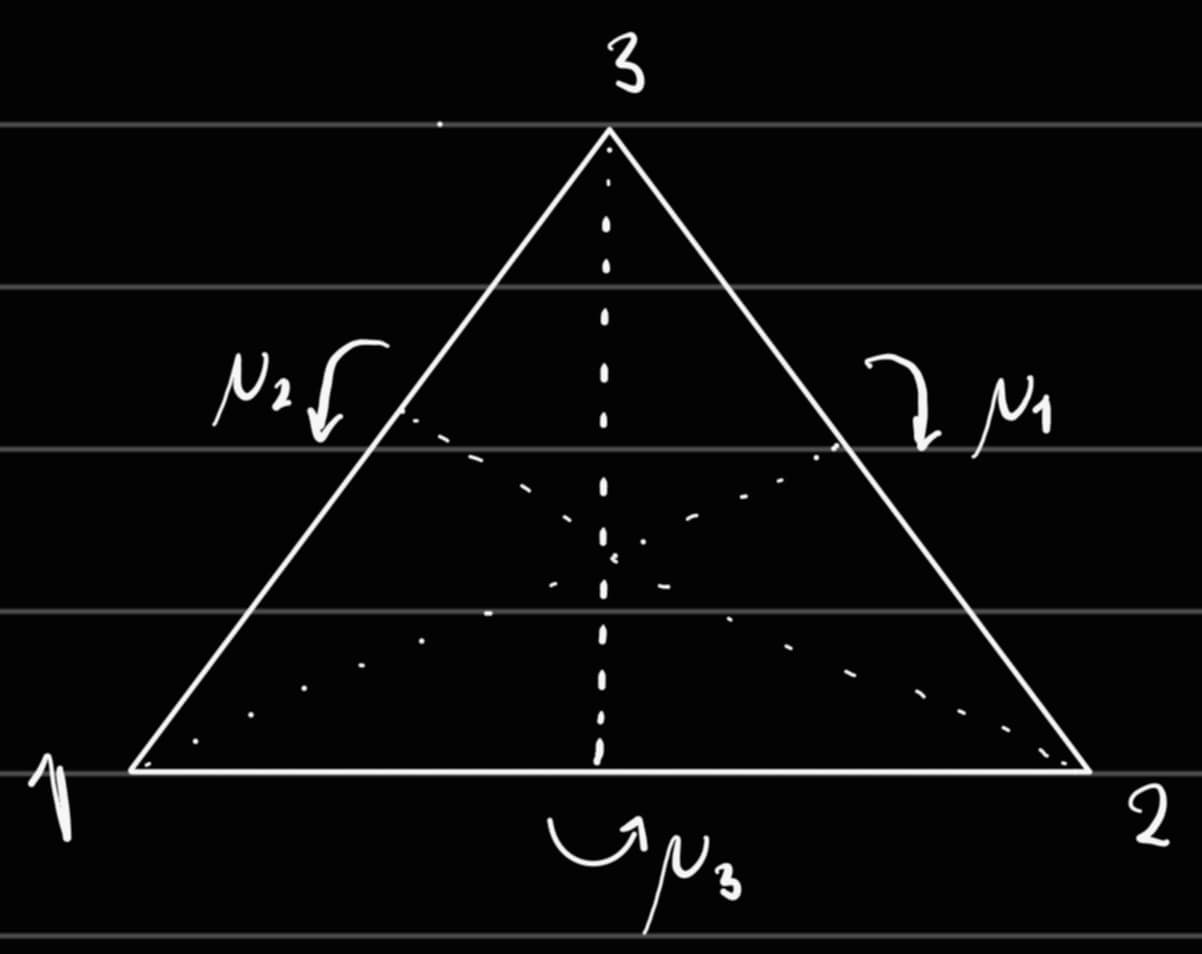
\includegraphics[width=0.5\textwidth]{images/symmetry_group_s3_illustration.jpg}
	\caption{Illustrasjon av $S_3$}
	\label{fig:symmetry-group-s3}
\end{figure}

Her definerer vi følgende elementer:
\begin{itemize}
	\item $\rho_0$: Rotasjon med $0^\circ$ mot klokken, som tilsvarer
	      $\begin{pmatrix}1 & 2 & 3 \\ 1 & 2 & 3\end{pmatrix}$
	\item $\rho_1$: Rotasjon med $120^\circ$ mot klokken, som tilsvarer
	      $\begin{pmatrix}1 & 2 & 3 \\ 2 & 3 & 1\end{pmatrix}$
	\item $\rho_2$: Rotasjon med $240^\circ$ mot klokken, som tilsvarer
	      $\begin{pmatrix}1 & 2 & 3 \\ 3 & 1 & 2\end{pmatrix}$
	\item $\mu_1$: Speiling om linje 1, som tilsvarer
	      $\begin{pmatrix}1 & 2 & 3 \\ 1 & 3 & 2\end{pmatrix}$
	\item $\mu_2$: Speiling om linje 2, som tilsvarer
	      $\begin{pmatrix}1 & 2 & 3 \\ 3 & 2 & 1\end{pmatrix}$
	\item $\mu_3$: Speiling om linje 3, som tilsvarer
	      $\begin{pmatrix}1 & 2 & 3 \\ 2 & 1 & 3\end{pmatrix}$
\end{itemize}

Binæroperasjonen i $S_3$ er komposisjon av permutasjoner, men dette svarer til komposisjon av
symmetrier.

\textbf{Eksempel}:
Vi har at
\begin{align}
	\mu_3\rho_2 & =\begin{pmatrix}1 & 2 & 3 \\ 2 & 1 & 3\end{pmatrix}
	\begin{pmatrix}1 & 2 & 3 \\ 3 & 1 & 2\end{pmatrix}                 \\
	            & = \begin{pmatrix}1 & 2 & 3 \\ 3 & 2 & 1\end{pmatrix} \\
	            & = \mu_2
\end{align}

\subsubsection{Multiplikasjonstabell til $S_3$}
Følgende er multiplikasjonstabellen til den tredje symmetrigruppen:

\[
	\begin{array}{c||cccccc}
		*      & \rho_0 & \rho_1 & \rho_2 & \mu_1 & \mu_2 & \mu_3 \\
		\hline\hline
		\rho_0 & \rho_0 & \rho_1 & \rho_2 & \mu_1 & \mu_2 & \mu_3 \\
		\rho_1 & \rho_1 & \rho_2 & \rho_0 & \mu_3 & \mu_1 & \mu_2 \\
		\rho_2 & \rho_2 & \rho_0 & \rho_1 & \mu_2 & \mu_3 & \mu_1 \\
		\mu_1  & \mu_1 & \mu_2 & \mu_3 & \rho_0 & \rho_1 & \rho_2 \\
		\mu_2  & \mu_2 & \mu_3 & \mu_1 & \rho_2 & \rho_0 & \rho_1 \\
		\mu_3  & \mu_3 & \mu_1 & \mu_2 & \rho_1 & \rho_2 & \rho_0 \\
	\end{array}
\]

\textbf{Undergrupper}:
\begin{itemize}
  \item $\cb{\rho_0}$
  \item $\cb{\rho_0, \rho_1, \rho_2}=\inner{\rho_1}=\inner{\rho_2}$
  \item $\cb{\rho_0, \mu_i}_{i=1,2,3}$
  \item $S_3$ selv, som ikke er syklisk
\end{itemize}

\section{Baner, Sykler og $A_n$}

\begin{definition}{Banen til et element}{}
  La $A$ være en mengde, $\sigma\in S_A$ og $a\in A$. Da sier vi at \textbf{banen} til $a$ er
  \begin{align}
    \cb{\sigma^n(a)\mid n\in \mathbb{Z}}\subset A
  \end{align}
\end{definition}

\textbf{Eksempel}:
La
\begin{align}
  \sigma=\begin{pmatrix}1 & 2 & 3 & 4 & 5 & 6 \\ 5 & 1 & 6 & 4 & 2 & 3\end{pmatrix}\in S_6
\end{align}
Da ser vi at 
\begin{align}
  \sigma(1)&=5 \\
  \sigma^2(1)&=2 \\
  \sigma^3(1)&=1 \\
  \sigma^4(1)&=5 
\end{align}
noe som betyr at $\cb{1, 2, 5}$ er banen til 1, 2 og 5. Videre ser vi at 
\begin{align}
  \sigma(3)&=6 \\
  \sigma^2(3)&=3
\end{align}
som betyr at $\cb{3, 6}$ er banen til 3 og til 6. Til slutt så ser vi at
\begin{align}
  \sigma(4)=4
\end{align}
som betyr at $\cb{4}$ er banen til 4. 

\begin{definition}{Sykel}{}
  $\sigma\in S_n$ er en \textbf{sykel} hvis det maksimalt er en bane med mer enn et element. 
\end{definition}

\textbf{Eksempel}: Se på 
$\tau=\begin{pmatrix}1 & 2 & 3 & 4 & 5 6 \\ 1 & 2 & 6 & 4 & 5 & 3\end{pmatrix}\in S_6$. Denne
permutasjonen har banene
\begin{align}
  \cb{1}, \cb{2}, \cb{4}, \cb{5}, \cb{3, 6}
\end{align}
Dermed er $\tau$ en sykel, mens $\sigma$ fra over ikke er det.

\textbf{Merk}:
\begin{enumerate}
  \item Vi bruker notasjonen $\tau=\nb{3, 6}$ for $\tau$ definert som over
  \item La $\mu=(1,5,2)$ og $\tau=(3,6)$ i $S_6$. Altså at
    \begin{align}
      \mu &= \begin{pmatrix}1 & 2 & 3 & 4 & 5 & 6 \\ 5 & 1 & 3 & 4 & 2 & 6\end{pmatrix} \\
      \tau &= \begin{pmatrix}1 & 2 & 3 & 4 & 5 & 6 \\ 1 & 2 & 6 & 4 & 5 & 3\end{pmatrix} 
    \end{align}
    Da er $\mu\tau=\sigma=\tau\mu$ (vis)
\end{enumerate}

\begin{theorem*}{9.8}{}
  Ethvert element i $S_n$ er et produkt av sykler. 
\end{theorem*}

\begin{definition}{Transposisjon}{}
  En sykel av lengde 2 er en \textbf{transposisjon}.
\end{definition}

\textbf{Merk}: La $(a_1, a_2, \ldots, a_t)$ være en sykel i $S_n$. Da er
\begin{align}
  (a_1, a_2, \ldots, a_t)=(a_1, a_t)(a_1, a_{t-1})\cdots(a_1,a_2)
\end{align}

\textbf{Eksempel}: I $S_6$ så er $(1, 5, 2)=(1,2)(1,5)$ og i $S_{39}$ så er 
$(2,8,13,38)=(2,38)(2,13)(2,8)$

\begin{theorem*}{(Korollar) 9.12}{}
  Ethvert element i $S_n$ er et produkt av transposisjoner.
\end{theorem*}

\textbf{Eksempler}:
\begin{enumerate}
  \item $\sigma$ fra eksempelet tidligere kan skrives som: 
    $\sigma=(1,5,2)(3,6)=(1,2)(1,5)(3,6)$
  \item $(a,b)(a,b)$ blir til identiteten i $S_n$. F.eks. så har vi at $(1,2)(1,2)=\text{id}$.
  \item For $\sigma$ i punkt 1 så kan vi skrive
    \begin{align}
      \sigma=(1,2)(1,5)(3,6)=(1,2)(2,4)(2,4)(1,5)(3,6)
    \end{align}
    siden $(2,4)(2,4)$ blir identiteten. 
\end{enumerate}

\begin{theorem*}{9.15}{}
  Et element i $S_n$ kan ikke både skrives som et produkt av et odde antall transposisjoner og
  som et produkt av et partall antall transposisjoner.
\end{theorem*}

\begin{definition}{Like og Odde}{}
  Vi sier at $\sigma\in S_n$ er \textbf{like} dersom $\sigma$ er et produkt av et partall antall
  transposisjoner og \textbf{odde} dersom $\sigma$ er et produkt av et odde antall transposisjoner.
\end{definition}

\textbf{Eksempler}:
\begin{enumerate}
  \item $\sigma$ fra tidligere er odde siden $\sigma=(1,6)(1,5)(3,6)$.
  \item Identitetselementet i $S_n$ er like fordi det kan skrives som $(1,2)(1,2)$.
\end{enumerate}

\begin{theorem*}{9.20}{}
  For $n\geq 2$ la $A_n=\cb{\sigma\in S_n\mid\sigma\text{ er like}}$. Da er $A_n\leq S_n$ med
  $\abs{A_n}=\frac{\abs{S_n}}{2}=\frac{n!}{2}$.
\end{theorem*}

\textbf{Bevis}: Først så har vi at $A_n\neq\emptyset$ siden $n\geq 2$.

La 
\begin{align}
  \sigma=&(a_1,b_1)\cdots(a_{2s},b_{2s})\in A_n \\
  \tau=&(c_1,d_1)\cdots(c_{2t},d_{2t})\in A_n \\
\end{align}
Da har vi at
\begin{align}
  \sigma\tau^{-1}=\sb{(a_1,b_1)\cdots(a_{2s},b_{2s})}(c_{2t},d_{2t})\cdots(c_1,d_1)
\end{align}
som betyr at $\sigma\tau^{-1}$ kan skrives som et produkt av et partalls antall transposisjoner,
som igjen betyr at $\sigma\tau^{-1}$ må være like. Dermed er $\sigma\tau^{-1}\in A_n$, som
betyr at $A_n$ er en gyldig undergruppe av $S_n$. \qed

La $B_n=\cb{\sigma\in S_n\mid\sigma\text{ er odde}}$.

\begin{theorem*}{(Korollar) 9.12}{}
  $S_n=A_n\cup B_n$ 
\end{theorem*}

\begin{theorem*}{9.15}{}
  $A_n\cap B_n=\emptyset$ og $\abs{S_n}=\abs{A_n}+\abs{B_n}$. 
\end{theorem*}

\section{Restklasser og Lagranges Teorem}
I dette kapittelet kommer vi til å anta at $H\leq G$.

\textbf{Mål}:
\begin{enumerate}
	\item Vise at dersom $\abs{G}<\infty$ så vil $\abs{H}\mid\abs{G}$.
	\item Etter hvert: Lage en ny gruppe $G/H$ for visse undergrupper $H$.
\end{enumerate}

\begin{definition}{Restklasse}{}
	La $a\in G$. Da er $Ha=\cb{ha\mid h\in H}$ den \textbf{høyre restklassen} til $H$ mhp. $a$, og
	$aH=\cb{ah\mid h\in H}$ den \textbf{venstre restklassen} til $H$ mhp. $a$.

	Dersom $G$ er abelsk så er $Ha=aH\ \forall a\in G$.
\end{definition}

\textbf{Eksempler}:

\begin{enumerate}
	\item La $G=\mathbb{Z}$ og $H=5 \mathbb{Z}=\cb{\dots,-10,-5,0,5,10,\dots}$. Da finnes det
	      fem restklasser:
	      \begin{align}
		      0 + 5 \mathbb{Z} & = 5 \mathbb{Z}                    \\
		      1 + 5 \mathbb{Z} & = \cb{\dots, -9, -4, 1, 6, \dots} \\
		      2 + 5 \mathbb{Z} & = \cb{\dots, -8, -3, 2, 7, \dots} \\
		      3 + 5 \mathbb{Z} & = \cb{\dots, -7, -2, 3, 8, \dots} \\
		      4 + 5 \mathbb{Z} & = \cb{\dots, -6, -1, 4, 9, \dots} \\
		      5 + 5 \mathbb{Z} & = 5 \mathbb{Z}                    \\
		      6 + 5 \mathbb{Z} & = 1+5 \mathbb{Z}
	      \end{align}
	\item La $U_4=\cb{1,-1,i,-i}$ med multiplikasjon og $H={-1,1}$. Da har vi følgende
	      restklasser:
	      \begin{align}
		      H\cdot 1 & = H\cdot(-1) = H          \\
		      H\cdot i & = H\cdot(-i) = \cb{-i, i} 
	      \end{align}
        Så det finnes totalt to restklasser
      \item La $G=S_3=\cb{\rho_0, \rho_1, \rho_2, \mu_1, \mu_2, \mu_3}$ og $H=\cb{\rho_0, \mu_1}$.
        Da ser vi at:
        \begin{align}
          H\rho_1 &= \cb{\rho_1, \mu_2} \\
          \rho_1 H &= \cb{\rho_1, \mu_3}
        \end{align}
        Så vi ser at $H\rho_1\neq\rho_1 H$. 
\end{enumerate}

\textbf{Merk (for både høyre og venstre restklasser)}:
\begin{enumerate}
  \item $a\in Ha$ fordi $ea=a$
  \item $Ha=H\iff a\in H$. 

    Dersom $Ha=H$ så er $a\in H$ fra punkt 1. Dersom $a\in H$ så er $Ha\subseteq H$ siden
    $H$ er lukket. La nå $h\in H$. Da kan vi skrive $h=(ha^{-1})a$, men $ha^{-1}\in H$, så
    $h\in Ha$. \qed
  \item $Ha\cap Hb\neq\emptyset\iff Ha=Hb$. Her er $\impliedby$-retningen triviell. 

    Hvis $Ha\cap Hb\neq\emptyset$ så finnes $h_1,h_2\in H$ slik at $h_1a=h_2b$. Dette gir oss
    at $a=h_1^{-1}h_2b$. Dermed har vi at for $h\in H$ så er $ha=(hh_1^{-1}h_2)b\in Hb$.
    Siden vi valgte $h$ vilkårlig så må da $Ha\subseteq Hb$. Vi kan bruke et tilsvarende
    argument for å see at $Hb\subseteq Ha$, noe som betyr at $Hb=Ha$. \qed
  \item $Ha=Hb\iff ab^{-1}\in H\iff ba^{-1}\in H$. 

    Vi ser at $Ha=Hb\iff Hab^{-1}=Hbb^{-1}\iff Hab^{-1}=H\iff ab^{-1}\in H$, hvor vi i det siste
    steget brukte resultatet fra punkt 2.
  \item $Ha=Hb\iff b\in Ha$ fra punkt 1 og 4.
  \item Definer $f:H\ra Ha$ ved $f(h)=ha$. Dette er en bijeksjon, så $\abs{H}=\abs{Ha}$.
\end{enumerate}

\begin{theorem*}{Lagrange}{}
Hvis $\abs{G}<\infty$ og $H\leq G$ så vil $\abs{H}$ være en divisor i $\abs{G}$.
\end{theorem*}

\textbf{Bevis}:
Fra resultatene over og siden $G$ er endelig så må det eksistere elementer 
$a_1, a_2, \dots, a_t\in G$ slik at 
\begin{enumerate}
  \item $G=Ha_1\cup Ha_2\cup \dots\cup Ha_t$
  \item $Ha_i\cap Ha_j=\emptyset$ for alle $i\neq j$ (siden alle restklassene er disjunkte eller 
    fullstendig overlappende)
\end{enumerate}
Så siden $\abs{Ha_i}=\abs{H}$ så må $\abs{G}=t\abs{H}$. \qed

\begin{theorem*}{(Korollar) 10.11}{}
  Anta $\abs{G}=p$ hvor $p$ er et primtall. Da har $G$ kun to undergrupper, $\cb{e}$ og $G$ selv.

  Dersom $a\neq e$ så vil $\inner{a}=G$. Spesielt er $G$ syklisk og $G$ er isomorf med
  $\mathbb{Z}_p$.
\end{theorem*}

\textbf{Eksempel} (Vår 2012, oppgave 1): 
La $G$ være en gruppe som inneholder minst ett element av orden 3 og minst ett av orden 4. Hva er
den minste ordenen en slik gruppe kan ha og gi et eksempel.

Siden 3 må dele ordenen og 4 må dele ordenen til gruppen så ma $3\cdot 4$ også dele ordenen,
så ordenen må minst være 12. Et eksempel på en slik gruppe er $\mathbb{Z}_{12}$.

\begin{definition}{Indeks}{}
  Vi sier at \textbf{indeksen} til $H$ i $G$ er $(G:H)=$ antall ulike høyre restklasser til $H$
  (som er det samme som antall venstre restklasser).
\end{definition}

\textbf{Eksempel}: $(\mathbb{Z}:5 \mathbb{Z})=5$.

\textbf{Merk}: Når $\abs{G}<\infty$ så er $(G:H)=\frac{\abs{G}}{\abs{H}}$.


\section{Produkt av grupper}
Vi er kjente med at dersom $S_1, S_2, \dots, S_t$ er mengder, så er det kartesiske produktet
mellom de definert som
\begin{align}
	S_1\times S_2\times \cdots\times S_t = \cb{(s_1,s_2,\dots,s_t)\mid s_i\in S_i}
\end{align}

\textbf{Eksempel}:
\begin{align}
	\mathbb{Z}\times\mathbb{Z}\times\mathbb{C}=\cb{(x,y,z)\mid x,y\in\mathbb{Z}, z\in\mathbb{C}}
\end{align}

\textbf{Merk}: Vi har at
\begin{align}
	\abs{S_1\times S_2\times\cdots\times S_t}=\prod_{i=1}^t\abs{S_i}
\end{align}

\begin{theorem*}{11.2}{}
	La $G_1, \dots, G_t$ være grupper. Da har vi at $G_1\times\cdots\times G_t$ er en gruppe
	med binæroperasjon
	\begin{align}
		(a_1,\dots,a_t)(b_1,\dots,b_t)=(a_1b_1,\dots,a_tb_t)
	\end{align}
	hvor multiplikasjonen skjer elementvis og hører til hver enkelt gruppe. Dette er det
	\textbf{direkte produktet} av $G_1,\dots, G_t$.
\end{theorem*}

\textbf{Bevis}: Oppgave

\textbf{Merk}:
\begin{enumerate}
	\item Vi bruker $\prod_{i=1}^t G_i$ notasjon.
	\item Identitetselementet er $(e_1, e_2, \dots, e_t)$ hvor $e_i\in G_i$ er identiteten.
	\item Vi har at $(a_1, a_2, \dots, a_t)^{-1}=(a_1^{-1}, a_2^{-1},\dots, a_t^{-1})$
	\item Vi har at $\prod G_i$ er abelsk $\iff G_i$ er abelsk $\forall i$
\end{enumerate}

\textbf{Eksempler}:
\begin{enumerate}
	\item La oss se på $(\mathbb{Z}, +)$ og $(U,\cdot)$, hvor $U=\cb{z\in \mathbb{C}\mid\abs{z}=1}$.
	      Da har vi at binæroperasjonen til $\mathbb{Z}\times U$ er gitt ved $(a,z)(b,w)=(a+b,zw)$.
	\item $\mathbb{Z}_2\times \mathbb{Z}_2$ har fire elementer, $\cb{(0,0), (0,1), (1,0), (1,1)}$

	      Vi ser at $(1,0)+(1,0)=(1+1,0+0)=(0,0)$.

	      Elementene $(1,0)$, $(0,1)$ og $(1,1)$ har orden 2 i $\mathbb{Z}_2\times \mathbb{Z}_2$, så
	      ingen elementer har orden 4, altså finnes det ingen elementer som genererer hele grupper.
	      Dermed er den ikke syklisk.

	      Altså har vi at $\mathbb{Z}_4$ og $\mathbb{Z}_2\times \mathbb{Z}_2$ er ikke-isomorfe abelske
	      grupper med 4 elementer.
\end{enumerate}

\begin{theorem*}{11.5}{}
	$\mathbb{Z}_m\times \mathbb{Z}_n$ er syklisk (og dermed isomorf med $\mathbb{Z}_{mn}$)
	$\iff \gcd(m,n)=1$.
\end{theorem*}

\textbf{Bevis}: Anta at $\gcd{m,n}=1$. Vis da at $(1,1)$ genererer hele
$\mathbb{Z}_m\times \mathbb{Z}_n$

Motsatt, dersom $\gcd(m,n)=d\geq 2$, kan man vise at ingen elementer i gruppen genererer hele
gruppen.

Ordenen til $(a,b)\leq \frac{m\cdot n}{d}<m\cdot n$.

\begin{theorem*}{(Korollar) 11.6}{}
	$\mathbb{Z}_{n_1}\times\cdots\times \mathbb{Z}_{n_t}$ er syklisk (og isomorf med
	$\mathbb{Z}_{\prod_{i=1}^t n_i}$) $\iff \gcd(n_i, n_j)=1\ \forall i\neq j$
\end{theorem*}

\begin{theorem*}{11.9}{}
  La $G_1,\dots,G_t$ være grupper og $a_i\in G_i$ være elementer av orden $n_i$. Da har vi at
  $(a_1,\dots,a_t)$ har orden $\text{lcm}(n_1,n_2,\dots,n_t)$.
\end{theorem*}

\textbf{Eksempel}: Se på $\mathbb{Z}_5\times \mathbb{Z}_8$ og elementet $(2,3)$. Siden 
2 har orden 5 i $\mathbb{Z}_5$ og 3 har orden 8 i $\mathbb{Z}_8$, så har $(2,3)$
orden $\text{lcm}(5,8)=40$. Altså må $(2,3)$ være en generator.

Se på $(2,4)$. Siden $4$ har orden 2 i $\mathbb{Z}_8$ så har $(2,4)$ orden $\text{lcm}(5,2)=10$.


\begin{theorem*}{11.12 (Fundamentalteoremet for endeliggenererte abelske grupper)}{}
  Enhver endeliggenerert abelsk gruppe er isomorf med et direkte produkt på formen
  \begin{align}
    \mathbb{Z}_{p_1^{n_1}}\times\cdots\times \mathbb{Z}_{p_t^{n_t}}
    \times\mathbb{Z}\times\cdots\times \mathbb{Z}
  \end{align}
  hvor $p_i$ er primtall (men ikke nødvendigvis disinkte) og det er unikhet. Spesielt så har vi
  at dersom $G$ er en endelig abelsk gruppe så er $G$ isomorf med et direkte produkt på
  formen
  \begin{align}
    \mathbb{Z}_{p_i^{n_1}}\times\cdots\times \mathbb{Z}_{p_t^{n_t}}
  \end{align}
\end{theorem*}

\textbf{Bevis}: MA3201, Ringer og Moduler 

\textbf{Eksempel} (Eksamen vår 2021, oppgave 1):
La $G$ være en abelsk gruppe med $\abs{G}=72$. Hvilke grupper kan $G$ være isomorf med?

Vi har at $72=3^2 \cdot 2^3$. Da har vi fra fundamentalteoremet for endeliggenererte abelske
grupper at $G$ må være isomorf med en av følgende:
\begin{itemize}
  \item $\mathbb{Z}_{9}\times \mathbb{Z}_8\cong \mathbb{Z}_{72}$
  \item $\mathbb{Z}_{9}\times \mathbb{Z}_4\times \mathbb{Z}_2$
  \item $\mathbb{Z}_{9}\times \mathbb{Z}_2\times \mathbb{Z}_2\times \mathbb{Z}_2$
  \item $\mathbb{Z}_3\times \mathbb{Z}_3\times \mathbb{Z}_8$
  \item $\mathbb{Z}_3\times \mathbb{Z}_3\times \mathbb{Z}_4\times \mathbb{Z}_2$
  \item $\mathbb{Z}_3\times \mathbb{Z}_3\times \mathbb{Z}_2\times \mathbb{Z}_2\times \mathbb{Z}_2$
\end{itemize}

\section{Homomorfier}
La $G$ og $H$ være grupper.

\begin{definition}{Homomorfi}{}
	En funksjon $\phi:G\ra H$ er en (gruppe-)\textbf{homomorfi} dersom
	\begin{align}
		\phi(g_1g_2)=\phi(g_1)\phi(g_2)\ \forall g_1,g_2\in G
	\end{align}
\end{definition}

\textbf{Eksempler}
\begin{enumerate}
	\item La $e_H$ være identiteten i $H$ og sett $\phi(g)=e_H$ for alle $g\in G$. Da har vi at
	      \begin{align}
		      \phi(g_1g_2)=e_H=e_He_H=\phi(g_1)\phi(g_2)
	      \end{align}
	\item Fikser $a\in \mathbb{Z}$ og definer $\phi_a: \mathbb{Z}\ra \mathbb{Z}$ ved
	      $n \mapsto an$. Da har vi at
	      \begin{align}
		      \phi_a(m+n)=a(m+n)=am+an=\phi_a(m)+\phi_a(n)
	      \end{align}
	      Vis at enhver homomorfi $\phi: \mathbb{Z}\ra \mathbb{Z}$ er på formen $\phi_a$ for
	      $a\in \mathbb{Z}$. Når er $\phi_a$ en isomorfi?
	\item Definer $\phi: \text{GL}(n,\mathbb{R})\ra \mathbb{R}^*$ ved $\phi(M)=\det M$. Da har
	      vi at
	      \begin{align}
		      \phi(MN)=\det(MN)=\det(M)\det(N)=\phi(M)\phi(N)
	      \end{align}
	      som betyr at $\phi$ er en homomorfi.
	\item Definer $\phi:S_n\ra S_{n+1}$ ved
	      \begin{align}
		      \sigma=\begin{pmatrix}1 & \dots & n \\ \sigma_1 & \dots & \sigma_n\end{pmatrix}
		      \mapsto
		      \begin{pmatrix}1 & \dots & n & n+1 \\ \sigma_1 & \dots & \sigma_1 & n+1\end{pmatrix}
	      \end{align}
	      Vis at $\phi(\sigma\tau)=\phi(\sigma)\phi(\tau)$
	\item Se på $(\mathbb{R}, +)$ og $(U, \cdot)$ hvor $U=\cb{z\in\mathbb{C}\mid\abs{z}=1}$.
	      \begin{align}
		      \phi: \mathbb{R} & \ra U          \\
		      r                & \mapsto e^{ir}
	      \end{align}
	      Da har vi at $\phi(r+s)=e^{i(r+s)}=e^{ir}e^{is}=\phi(r)\phi(s)$.
\end{enumerate}


\begin{theorem*}{13.12}{}
	La $\phi:G\ra H$ være en homomorfi. Da har vi at følgende holder:
	\begin{enumerate}
		\item Dersom $e\in G$ er identitetselementer så er $\phi(e)$ identitetselementet i $H$
		\item $\phi(g^{-1})=\phi(g)^{-1}\ \forall g\in G$
		\item $K\leq G\implies \phi[K]=\cb{\phi(k)\mid k\in K}\leq H$
		\item $L\leq H\implies \phi^{-1}[L]=\cb{g\in G\mid \phi(g)\in L}\leq G$
	\end{enumerate}
	Med andre ord impliserer homomorfier en slags strukturbevaring.
\end{theorem*}

\textbf{Bevis}:
\begin{enumerate}
	\item Vi har at $\phi(e)=\phi(ee)=\phi(e)\phi(e)$. Gang nå med $\phi(e)^{-1}$ på begge sider.
	      Da får du $\phi(e)^{-1}\phi(e)=\phi(e)^{-1}\phi(e)\phi(e)\implies e_H=\phi(e)$. \qed
	\item Vi ser at
	      \begin{align}
		      e_H=\phi(e)=\phi(gg^{-1})=\phi(g)\phi(g^{-1})\implies \phi(g^{-1})=\phi(g)^{-1}\qed
	      \end{align}
\end{enumerate}

\begin{definition}{Kjernen}{}
	La $e_H$ være identitetselementet i $H$. Da er kjernen til $\phi$ definert som:
	\begin{align}
		\ker \phi = \cb{g\in G\mid \phi(g)=e_H}
	\end{align}
\end{definition}

\textbf{Merk}: $\ker \phi \leq G$. Dette kommer fra punkt 4 i teoremet over siden det inverse
bildet til $e_H$ vil være kjernen til $\phi$.

\textbf{Eksempler}: (Her bruker vi de samme eksemplene som over)
\begin{enumerate}
	\item $\ker\phi=G$
	\item $\ker\phi_a=\begin{cases}\cb{0} & a \neq 0 \\ \mathbb{Z} & a=0 \end{cases}$
	\item $\ker\phi = \text{SL}(n, \mathbb{R}) \leq \text{GL}(n, \mathbb{R})$
	\item $\ker\phi = \cb{\sigma\in S_n\mid \phi(\sigma)=\text{id}_{n+1}}=\cb{e}$
	\item Vi har at:
	      \begin{align}
		      \ker\phi & =\cb{a\in \mathbb{R}\mid \phi(a)=1}    \\
		               & =\cb{a\in \mathbb{R}\mid e^{ir}=1}     \\
		               & =\cb{n\cdot 2\pi \mid n\in \mathbb{Z}}
	      \end{align}
\end{enumerate}

\begin{theorem*}{(Korollar) 13.18}{}
	For en homomorfi $\phi:G\ra H$ så har vi at $\phi$ er injektiv hvis og bare hvis
	$\ker\phi=\cb{e}$.
\end{theorem*}

\textbf{Bevis}: La oss først anta at $\phi$ er injektiv og at $g\in G$ med $\phi(g)=e_H$. Siden
$\phi(e)=e_H$ og $\phi$ er injektiv, så må da $g=e_H$.

Anta nå at $\phi$ ikke er injektiv. Da må det finnes $g_1, g_2\in G$ slik at $g_1\neq g_2$
men $\phi(g_1)=\phi(g_2)$. Da har vi at
\begin{align}
	e_H & =\phi(g_1)\phi(g_1)^{-1} \\
	    & =\phi(g_2)\phi(g_1)^{-1} \\
      &= \phi(g_2)\phi(g_1^{-1}) \\
      &= \phi(g_2g_1^{-1}).
\end{align}

Legg merke til at $g_2g_1^{-1}\neq e$ siden inverser er unike. Dermed har vi vist at 
$\ker\phi\neq \cb{e}$, som var det vi ville vise. \qed

\section{Faktorgrupper}

\textbf{Mål}: For en gruppe $G$ og visse undergrupper $H\leq G$ så vil vi lage en ny gruppe
$G/H$ hvor elementene i $G/H$ er restklassene til $H$ i $G$.

\begin{definition}{Normal Undergruppe}{}
	Vi kaller en undergruppe $H\leq G$ \textbf{normal} dersom $gH=Hg\ \forall g\in G$.
\end{definition}

\textbf{Eksempler}:
\begin{enumerate}
	\item $H=\cb{e}\implies gH=\cb{g}=Hg$ for alle $g\in G$, så her er $H$ normal.
	\item Dersom $G$ er abelsk så er $H\leq G$ automatisk normal.
	\item La $G=S_3$ tolket som symmetrier på et triangel,
	      $\cb{\rho_0, \rho_1, \rho_2, \mu_1, \mu_2, \mu_3}$. Vi har tidligere sett at
	      $H=\cb{\rho_0, \rho_1, \rho_2}$ er en undergruppe. Vi har at $\rho_i H=H=H\rho_i$ siden
	      $\rho_i\in H$.

	      Vis at $\mu_i H=H\mu_i$.

	      Altså har vi at $H\leq G$ er en normal undergruppe.

	\item La oss fortsatt se på $S_3$, men sett nå $H=\cb{\rho_0, \mu_1}$. Da har vi at
	      $\rho_1 H=\cb{\rho_1, \mu_3}$, men at $H\rho_1 =\cb{\rho_1, \mu_2}$. Altså er ikke $H$
	      normal i dette tilfellet.
\end{enumerate}

\begin{theorem*}{14.12}{}
	Følgende er ekvivalent for $H\leq G$:
	\begin{enumerate}
		\item $H$ er normal
		\item $gHg^{-1}\ \forall g\in G$, hvor $gHg^{-1}=\cb{ghg^{-1}\mid h\in H}$
		\item $ghg^{-1}\in H\ \forall h\in H, g\in G$
	\end{enumerate}
\end{theorem*}

Fra tidligere så har vi:
\begin{enumerate}
	\item $g\in G$
	\item $gH=H\iff g\in H$
	\item $g_1H\cap g_2H\neq\emptyset\iff g_1H=g_2H\iff g_1^{-1}g_2\in H\iff g_2^{-1}g_1\in H\iff g_2\in g_1 H$
\end{enumerate}

\textbf{Eksempel}: La $G=S_3$. Da ser vi at
\begin{enumerate}
	\item $H=\cb{\rho_0, \rho_1, \rho_2}\implies \rho_1H=H$ og $\mu_i H=\cb{\mu_1, \mu_2, \mu_3}$
	\item La $H=\cb{\rho_1, \mu_1}$. Da ser vi at $\rho_1 H=\cb{\rho_1, \mu_3}$, altså at
	      $\mu_3\in \rho_1 H$, som må bety at $\rho_1 H=\mu_1 H$ (siden de enten er helt disjunkte
	      eller helt like).
\end{enumerate}

\begin{theorem*}{14.14 og korollar 14.5}{}
	Anta at $H\leq G$ er normal og la $G/H$ være mengden av restklasser til $H$ i $G$. For
	$g_1H$ og $g_2H$ i $G/H$, definer
	\begin{align}
		(g_1H)(g_2H)=(g_1g_2)H\in G/H
	\end{align}
	Dette er en binæroperasjon på $G/H$, som blir en gruppe sammen med denne.
\end{theorem*}

\textbf{Bevis}: Må vise at binæroperasjonen er veldefinert i følgende forstand: La
$g_1'\in g_1H$. Da vet vi at $g_1H=g_1'H$. Tilsvarende har vi at for $g_2'\in g_2H$ er
$g_2H=g_2'H$. Må vise
\begin{align}
	(g_1g_2)H=(g_1'g_2')H
\end{align}
Med andre ord så må vi vise at dersom to elementer i domenet er like så må de også ende opp
på samme sted i ko-domenet.

Siden $(g_1H)(g_2H)=(g_1'H)(g_2'H)$, så kan vi ta et element $g_1'g_2'h\in (g_1'g_2')H$. Siden
$g_1'\in g_1H$ og $g_2'\in g_2H$, så finnes $h_1, h_2\in H$ slik at $g_1'=g_1h_1$ og
$g_2'=g_2h_2$. Da har vi at
\begin{align}
	g_1'g_2'h & = (g_1h_1)(g_2h_2)h          \\
	          & = g_1(e)h_1g_2h_2h           \\
	          & = g_1(g_2g_2^{-1})h_1g_2h_2h \\
	          & = g_1g_2(g_2^{-1}h_1g_2)h_2h
\end{align}
Husk at siden $H$ er normal og $h_1\in H$, så må $g_2^{-1}h_1g_2\in H$. Dermed kan vi skrive
$\widetilde h := g_2^{-1}h_1g_2$. Videre har vi at $\widetilde{h}h_2h\in H$ siden $H$ er lukket.
Dermed får vi altså
\begin{align}
	g_1'g_2'h & = g_1g_2\widetilde{h}h_2h \in (g_1g_2)H
\end{align}
Derfor har vi at $(g_1'g_2')H\subseteq (g_1g_2)H$. Vi kan gjøre tilsvarende argument andre vei og
få $(g_1g_2)H\subseteq (g_1'g_2')H$, som tilsammen må bety at $(g_1g_2)H=(g_1'g_2')H$, som var
det vi ville vise. Dermed har vi vist at operatoren over er veldefinert.

La oss nå vise at dette blir en gruppe.
\begin{enumerate}[label=$\mathscr{G}$\arabic*)]
	\item Assosiativitet:
	      \begin{align}
		      g_1H\sb{(g_2H)(g_3H)} & = g_1H((g_2g_3)H)       \\
		                            & = g_1(g_2g_3)H          \\
		                            & = (g_1g_2)g_3H          \\
		                            & = \dots                 \\
		                            & = \sb{(g_1H)(g_2H)}g_3H
	      \end{align}
	\item Identitet: Vi har at $eH=H$ er identitetselementet:
	      \begin{align}
		      (eH)(gH)=(eg)H=gH=(ge)H=(gH)(eH)\ \forall g\in G
	      \end{align}
	\item Invers: Vi har at $(gH)^{-1}=g^{-1}H$:
	      \begin{align}
		      (gH)(g^{-1}H)=(gg^{-1})H=eH=(g^{-1}g)H=(g^{-1}H)(gH)
	      \end{align}
\end{enumerate}

\begin{definition}{Faktorgruppe/Kvotientgruppe}{}
	Dersom $G$ er en gruppe og $H$ er en normal undergruppe så kaller vi $G/H$ en
	\textbf{faktorgruppe} eller \textbf{kvotientgruppe}.
\end{definition}

\textbf{Merk}:
\begin{enumerate}
	\item Vi brukte at $H\leq G$ er normal for å få at binæroperasjonen er veldefinert.
	\item binæreoperatoren for faktorgrupper er rett og slett a gange sammen restklasser:
	      \begin{align}
		      (g_1H)(g_2H) & = \cb{g_1h_1g_2h_2\mid h_1, h_2\in H}            \\
		                   & = \cb{g_1g_2g_2^{-1}h_1g_2h_2\mid h_1, h_2\in H} \\
		                   & = \cb{g_1g_2h\mid h\in H}                        \\
		                   & = (g_1g_2)H
	      \end{align}
\end{enumerate}

\textbf{Eksempler}:
\begin{enumerate}
	\item La $G=\mathbb{Z}$ og see på $H=4 \mathbb{Z}$. Vi har at $H$ her er normal siden
	      $\mathbb{Z}$ er en abelsk gruppe. Den har fire restklasser:
	      \begin{align}
		       & 0+4 \mathbb{Z} = 4 \mathbb{Z} \\
		       & 1+4 \mathbb{Z}                \\
		       & 2+4 \mathbb{Z}                \\
		       & 3+4 \mathbb{Z}
	      \end{align}
	      som også er de fire elementene i $\mathbb{Z}/4 \mathbb{Z}$. La oss se på addisjon i
	      $\mathbb{Z}/4 \mathbb{Z}$:
	      \begin{align}
		      (1+4 \mathbb{Z}) + (2+4 \mathbb{Z}) & = (1+2)+4 \mathbb{Z} = 3+4 \mathbb{Z}                  \\
		      (0+4 \mathbb{Z}) + (2+4 \mathbb{Z}) & = (0+2)+4 \mathbb{Z} = 2+4 \mathbb{Z}                  \\
		      (2+4 \mathbb{Z}) + (2+4 \mathbb{Z}) & = (2+2)+4 \mathbb{Z} = 0+4 \mathbb{Z} = 4 \mathbb{Z}   \\
		      (3+4 \mathbb{Z}) + (2+4 \mathbb{Z}) & = (3+2)+4 \mathbb{Z} = 5+4 \mathbb{Z} = 1+4 \mathbb{Z} \\
	      \end{align}
	      Merk her at $-(2+4 \mathbb{Z}) = 2 + 4 \mathbb{Z}$, altså at dette er inversen siden
	      $4 \mathbb{Z}$ er identiteten. Vi ser at $\abs{\mathbb{Z}/4 \mathbb{Z}}=4$ og at dette
	      ligner på $(\mathbb{Z}_4,+_4)$!
	\item La nå $G=S_3$ hvor vi ser på $H=\cb{\rho_0, \rho_1, \rho_2}$. Vi har allerede sett
	      at denne er normal. Det finnes to elementer i $S_3/H$:
	      \begin{itemize}
		      \item $H=\rho_0 H=\cb{\rho_0, \rho_1, \rho_2}=\rho_1 H=\rho_2 H$
		      \item $\mu_1 H = \cb{\mu_1, \mu_2, \mu_3}=\mu_2 H=\mu_3 H$
	      \end{itemize}
	      Altså har vi at $\abs{S_3/H}=2$ med $\rho_0 H$ som identitetselement og
	      $(\mu_1 H)(\mu_2 H)= \mu_1^2 H = \rho_0 H$. Dette ligner på $(\mathbb{Z}_2, +_2)$!
\end{enumerate}

\textbf{Merk}:
\begin{enumerate}
	\item Dersom $\phi:G\ra G'$ er en homomorfi så er $\ker\phi$ normal i $G$.
	\item $\phi[G]:= \cb{\phi(g)\mid g\in G}\leq G'$. Vi har også trivielt at $\phi:G\ra \phi[G]$
	      er en surjektiv homomorfi.
\end{enumerate}

Fra dette får vi at dersom $H\leq G$ er normal så kan vi lage følgende homomorfi:
\begin{align}
	\Pi : G & \ra G/H    \\
	g       & \mapsto gH
\end{align}
Da ser vi at $\Pi(g_1g_2)=g_1g_2H=(g_1H)(g_2H)=\Pi(g_1)\Pi(g_2)$. Videre har vi at
\begin{align}
	\ker\Pi = \cb{g\in G\mid \Pi(g)=eH}=\cb{g\in G\mid g\in H} = H
\end{align}

\begin{theorem*}{14.11 - Fundamentalteoremet for (gruppe-)homomorfier}{}
	La $\phi: G\ra G'$ være en homomorfi og $H=\ker\phi$. Da er funksjonen
	\begin{align}
		\bar\phi : G/H & \ra \phi[G]     \\
		gH             & \mapsto \phi(g)
	\end{align}
	en veldefinert homomorfi og en isomorfi. Videre har vi at $\phi = \bar\phi \circ \Pi$.
\end{theorem*}

\textbf{Bevis}:
\begin{itemize}
	\item Veldefinert:
	      \begin{align}
		      g_1H=g_2H & \implies g_2\in g_1H                                          \\
		                & \implies g_2=g_1h                                             \\
		                & \implies \bar\phi(g_2H)=\phi(g_2)=\phi(g_1h)=\phi(g_1)\phi(h)
		      =\phi(g_1)=\bar\phi(g_1)
	      \end{align}
	\item Homomorfi:
	      \begin{align}
		      \bar\phi((g_1H)(g_2H)) & = \bar\phi((g_1g_2)H)          \\
		                             & = \phi(g_1g_2)                 \\
		                             & = \phi(g_1)\phi(g_2)           \\
		                             & = \bar\phi(g_1H)\bar\phi(g_2H)
	      \end{align}
	\item Bijektiv: Vis
	\item Kommutativt diagram:
	      \begin{align}
		      (\bar\phi \circ \Pi)(g) & = \bar\phi(\Pi(g)) \\
		                              & = \bar\phi(gH)     \\
		                              & = \phi(g)
	      \end{align}
	      som var det vi ville vise. \qed
\end{itemize}

\textbf{Eksempler}:
\begin{enumerate}
	\item Se på $\phi: \mathbb{Z}\ra \mathbb{Z}_4$ med $n\mapsto n\pmod{4}$. Dette er en homomorfi.
	      $\phi$ er surjektiv og $\ker\phi=\cb{n\in \mathbb{Z}\mid n \equiv 0 \pmod{4}}=4 \mathbb{Z}$.
	      Da følger det fra teoremet over at $\mathbb{Z}/4 \mathbb{Z} \ra \mathbb{Z}_4$ er en isomorfi
	      ved $\bar\phi$.
	\item Se på $\phi: \text{GL}(n, \mathbb{R})\ra \mathbb{R}^*$ ved $\phi(M)=\det M$. Dette er en
	      homomorfi som er surjektiv med $\ker\phi=\text{SL}(n, \mathbb{R})$. Så
	      $\bar\phi: \text{GL}(n, \mathbb{R})/\text{SL}(n, \mathbb{R})\ra \mathbb{R}^*$ er en
	      isomorfi.
	\item Se på
	      \begin{align}
		      \phi:S_n & \ra \mathbb{Z}_2                                                                \\
		      \sigma   & \mapsto \begin{cases}0 & \sigma\text{ like}\\1 & \sigma \text{ odde}\end{cases}
	      \end{align}
	      Da er $\phi$ en surjektiv homomorfi og $\ker\phi=A_n$. Så $S_n/A_n\ra \mathbb{Z}_2$ er
	      en isomorfi.
	\item Vi ser at $G/\cb{e}\cong G$ med $\phi(g)=g$ og $G/G\cong \cb{e}$ med $\phi(g)=e$.
\end{enumerate}

\textbf{Strategi for å vise at $G/H$ er isomorf med en gruppe $G'$}:
\begin{enumerate}
	\item Finn en surjektiv homomorfi $\phi: G\ra G'$ med $\ker\phi=H$
	\item Da gir funtamentalteoremet oss at $G/H\ra G'$ er en isomorfi siden $\phi[G]=G'$.
\end{enumerate}

\textbf{Eksempel - Eksamen Sommer 2023, oppgave 4}:
La $G$ være en endelig gruppe og $H_1, H_2\leq G$ normale undergrupper.
\begin{enumerate}[label=\alph*)]
	\item La $\phi: G\ra G/H_1\times G/H_2$ med $\phi(g)=(gH_1,gH_2)$. Vis at $\phi$ er en homomorfi.

	      Løsning:
	      \begin{align}
		      \phi(g_1g_2) & = (g_1g_2H_1, g_1g_2H_2)              \\
		                   & = ((g_1H_1)(g_2H_1),(g_1H_2)(g_2H_2)) \\
		                   & = (g_1H_1,g_1H_2)(g_2H_1,g_2H_2)      \\
		                   & = \phi(g_1)\phi(g_2)
	      \end{align}
	      Så $\phi$ er en homomorfi.
	\item Finn en injektiv homomorfi
	      \begin{align}
		      G/(H_1\cap H_2)\ra G/H_1\times G/H_2
	      \end{align}
	      og vis at denne er en isomorfi hvis og bare hvis
	      \begin{align}
		      \frac{\abs{H_1}\abs{H_2}}{\abs{H_1\cap H_2}} = \abs{G}
	      \end{align}

	      Løsning:
        \begin{align}
          \ker\phi &= \cb{g\in G\mid \phi(g) = e} \\
                   &= \cb{g\in G\mid \phi(g)=(H_1, H_2)} \\
                   &= \cb{g\in G\mid g\in H_1 \wedge g\in H_2} \\
                   &= \cb{g\in G\mid g\in H_1\cap H_2} \\
                   &= H_1\cap H_2
        \end{align}
        Fra fundamentalteoremet har vi da at $\bar\phi: G/H_1\cap H_2 \ra \phi[G]$ er en
        isomorfi. Men merk at $\phi[G]\subseteq G/H_1 \times G/H_2$, så vi kan ikke garantere
        at $\bar\phi: G/H_1\cap H_2 \ra G/H_1\times G/H_2$ er surjektiv. Den må likevel
        være injektiv, siden isomorfien er det. Vi har at
        \begin{align}
          \phi \text{ surjektiv} &\iff \abs{G/H_1\cap H_2} = \abs{G/H_1\times G/H_2} \\
                                 &\iff \frac{\abs{G}}{\abs{H_1\cap H_2}} 
                                 =\frac{\abs{G}}{\abs{H_1}}\cdot \frac{\abs{G}}{\abs{H_2}} \\
                                 &\iff \frac{\abs{H_1}\abs{H_2}}{\abs{H_1\cap H_2}}
                                 = \frac{\abs{G}^2}{\abs{G}} = \abs{G} \qed
        \end{align}
\end{enumerate}

\begin{definition}{Simpel}{}
  Vi sier at en gruppe $G$ er \textbf{simpel} dersom det ikke finnes en normal undergruppe $H$ 
  slik at 
  \begin{align}
    \cb{e}<H<G
  \end{align}
\end{definition}

\textbf{Eksempel}: Dersom $\abs{G}=p$ hvor $p$ er et primtall så vet vi fra lagrange at 
$G$ må være simpel, siden det ikke kan finnes noen undergrupper $H$ med $\cb{e}<H<G$. 

\begin{theorem*}{15.15}{}
 $A_n$ er simpel når $n\geq 5$. 
\end{theorem*}

\begin{theorem*}{Klassifisering av endelige simple grupper}{}
 La $G$ være en endelig, simpel gruppe. Da er den isomorf med en av følgende:
 \begin{enumerate}
   \item $\mathbb{Z}_p$ hvor $p$ er et primtall
   \item $A_n$ når $n\geq 5$
   \item En simpel gruppe av Lie-type
   \item En av de 26 sporadiske gruppene
 \end{enumerate}
\end{theorem*}

\section{Gruppevirkninger}
\begin{definition}{Gruppevirkning}{}
	La $G$ være en gruppe og $X$ være en mengde. En \textbf{gruppevirkning} på $X$ fra
	$G$ er en funksjon $G\times X \ra X$ som tilfredsstiller to krav:
	\begin{itemize}
		\item $(e, x) = x$ for alle $x \in X$.
		\item $(g_1g_2, x) = (g_1, (g_2, x))$ for alle $g_1, g_2 \in G, x\in X$.
	\end{itemize}
	Dersom disse kravene tilfredsstilles så kaller vi $X$ en \textbf{$G$-mengde}.
	\newline\newline
	\textbf{Notasjon}: Dersom $g\in G$ og $x\in X$ så skriver vi normalt sett
	$(g, x) = gx$.
\end{definition}

\textbf{Eksempler}:
\begin{enumerate}
	\item La $G = S_n$ og $X = \cb{1, \dots, n}$. For en permutasjon $\sigma \in G$ og
	      $x\in X$ så er $\sigma x = \sigma(x)$ en gruppevirkning.
	\item La $G$ være en gruppe og $X=\cb{H\leq G}$ være mengden av alle undergrupper av
	      $G$. La oss videre definere en funksjon
	      \begin{align}
		      G\times X   & \ra X                                       \\
		      gH = (g, H) & \mapsto gHg^{-1} = \cb{ghg^{-1}\mid h\in H}
	      \end{align}
	      Sjekk at dette er en undergruppe av $G$. Vi har at $eH = eHe^{-1} = H$ og at
	      $(g_1g_2)H = g_1g_2Hg_2^{-1}g_1^{-1} = g_1(g_2Hg_2^{-1})g_1^{-1} = g_1(g_2H)$.
	      Denne gruppevirkningen kalles \textbf{Konjugasjon}.
	\item La
	      \begin{align}
		      G & = \cb{A\in \mathcal{M}_3(\mathbb{R})\mid A \text{ er ortogonal}} \\
		        & = \cb{A\in \mathcal{M}_3(\mathbb{R})\mid A^{-1} = A^\intercal}   \\
		        & = \text{O}_3(\mathbb{R})
	      \end{align}
	      være en gruppe med matrisemultiplikasjon som binæroperator. Merk at
	      $\norm{Av} = \norm{v} \forall v\in \mathbb{R}^3, A\in G$, altså at
	      $A$ bevarer normen til vektorer. Fiksér en $a > 0$ og la
	      $X = \cb{r\in \mathbb{R}^3\mid \norm{r} = a}$. For $A \in G$ og $v\in X$
	      så er $\norm{Av} = \norm{v}$, så $Av\in X$.

	      Videre har vi at:
	      \begin{enumerate}
		      \item $Iv = v \forall v\in X$
		      \item $(AB)v = A(Bv)\ \forall A, B\in G, v\in X$
	      \end{enumerate}
	      Dermed følger det at $X$ er en $G$-mengde og at vi har en gruppevirkning.
	\item La $G = \mathbb{Z}_2$ og $X = \mathbb{R}$. Definer så
	      \begin{align}
		      G\times X & \ra X                \\
		      mx        & \mapsto \begin{cases}
			                          x  & m = 0 \\
			                          -x & m = 1
		                          \end{cases}
	      \end{align}
	      Da er $0x = x$ og (sjekk) $(m + n)x = m(nx)$.
\end{enumerate}

\begin{definition}{Transitiv Virkning}{}
	La $G$ være en gruppe og $X$ en mengde. Vi sier at $G$ virker \textbf{transitivt} på
	$X$ dersom $\forall x_1, x_2\in X\ \exists g\in G$ hvor $gx_1 = x_2$.
\end{definition}

\textbf{Eksempel}: Vi har at (1) og (3) fra det forrige eksempelet er transitive virkninger.
Spesielt så ser vi at $forall v_1, v_2 \in \mathbb{R}^3$ med $\norm{v_1}=\norm{v_2}$ så vil det
finnes en $A \in \text{O}_3(\mathbb{R})$ slik at $Av_1 = v_2$ (ikke helt trivielt).

Videre har vi at (2) ikke er transitiv. Vi ser at $\abs{H} = \abs{gHg^{-1}}$, så derfor kan man
ikke gå fra en størrelse til en annen.

\begin{definition}{}{}
	La $G$ være en gruppe og $X$ en mengde, og la $g\in G$ og $x\in X$. Da definerer vi følgende
	mengder:
	\begin{align}
		G_x & = \cb{h\in G\mid hx = x} \subseteq G  \\
		X_g & = \cb{y \in X\mid gy = y} \subseteq X
	\end{align}
\end{definition}

\begin{theorem*}{}{}
	La $G$ være en gruppe, $X$ være en mengde og $x \in X$. Da vil $G_x \leq G$.
\end{theorem*}

\textbf{Bevis}:
La oss først merke at $G_x \neq \emptyset$ siden $e \in G_x$. La nå $h_1, h_2 \in G_x$. Da er
$h_i x = x$, noe som betyr at $x = h_i^{-1}x$. Da vil
\begin{align}
	(h_1h_2^{-1})x & = h_1(h_2^{-1}x) \\
	               & = h_1(x)         \\
	               & = x
\end{align}
noe som betyr at $h_1h_2^{-1} \in G_x$. Altså må $G_x \leq G$. \qed

\begin{definition}{Isotropi-undergruppen}{}
	$G_x$ kalles \textbf{isotropi-undergruppen} til $x$ i $G$.
\end{definition}

\begin{definition}{Bane til element in mengde}{}
	La $G$ være en gruppe, $X$ være en mengde og $x \in X$. Da sier vi at \textbf{banen} til $x$
	er $Gx = \cb{gx\mid g\in G}$.
\end{definition}

\textbf{Eksempler}:
\begin{enumerate}
	\item La $G$ være en gruppe og definer $X = \cb{H \leq G}$. Da vet vi at $g\cdot H = gHg^{-1}$
	      for $H\in X$. Da er $G_H = \cb{g\in G\mid gHg^{-1} = H}$.
	\item La $G = \text{O}_3(\mathbb{R})$ og $X = \cb{v\in \mathbb{R}^3\mid \norm{v} = a}$. Da har
	      vi at
	      \begin{align}
		      G_v & = \cb{A\in \text{O}_3(\mathbb{R})\mid Av = v} \\
		          & = \cb{A\in\text{O}_3(\mathbb{R})\
			      |\ v \text{ egenvektor av }A\text{ med }\lambda=1}
	      \end{align}
	\item Vi har at 'transitiv virkning $\iff Gx=X\ \forall x\in X$'
\end{enumerate}

\begin{theorem*}{16.16}{}
	La $G$ være en gruppe, $X$ være en mengde og $x\in X$ et element. Da har vi at
	$\abs{Gx} = (G:G_x)$, hvor $(G:G_x)$ betegner indeksen til $G_x$ i $G$, altså antall venstre
	restklasser.
\end{theorem*}
\textbf{Bevis}:
For $g_1, g_2\in G$ så har vi at 
$g_1x = g_2x \iff g_2^{-1}g_1x = x \iff g_2^{-1}g_1\in G_x \iff g_1G_x = g_2G_x$. Dermed har vi
altså en veldefinert funksjon:
\begin{align}
  Gx &\ra \cb{\text{venstre restklasser til }G_x\text{ i }G} \\
  gx &\mapsto gG_x
\end{align}
Ettersom denne funksjonen er bijektiv så må mengdene være like store, som var det vi ville 
vise. \qed

Vis følgende:
\begin{enumerate}
  \item $\forall x_1, x_2 \in X, x_1 \in Gx_2 \iff Gx_1 = Gx_2 \iff x_2 \in Gx_1$
  \item Definer relasjonen på $X$ ved $x_1 \in Gx_2$. Dette er en ekvivalensrelasjon.
  \item De følgende utsagnene er ekvivalente:
    \begin{enumerate}
      \item $G$ virker transitivt på $X$
      \item $Gx = X\ \forall x\in X$
      \item Det finnes $x\in X$ med $Gx = X$
      \item $X$ har kun én ekvivalensklasse for relasjonen i 2)
    \end{enumerate}
\end{enumerate}

\subsection{Burnsides Formel}

\begin{theorem*}{Burnsides Formel}{}
  La $G$ være en endelig gruppe og $X$ en endelig $G$-mengde med $r$ baner i $X$. Da følger det at:
  \begin{align}
    r\cdot \abs{G} = \sum_{g\in G}\abs{X_g}
  \end{align}
\end{theorem*}

\textbf{Bevis}: Se på undermengden $M$ av $G\times X$:
\begin{align}
  M = \cb{(g,x)\mid gx=x}
\end{align}
Da har vi at 
\begin{align}
  \sum_{g\in G}\abs{X_g} &= \sum_{g\in G}\abs{\cb{x\in X\mid gx=x}} = \abs{M} \\
                         &= \sum_{x\in X}\abs{\cb{g\in G\mid gx=x}} \\
                         &= \sum_{x_in X}\abs{G_x}
\end{align}
Videre har vi at for alle $x\in X$ så er $\abs{Gx} = (G:G_x) = \frac{\abs{G}}{\abs{G_x}}$. Da
må vi ha at 
\begin{align}
  \abs{M} &= \sum_{x\in X}\abs{G_x} = \sum_{x\in X}\frac{\abs{G}}{\abs{Gx}} 
          = \abs{G}\cdot \sum_{x\in X} \frac{1}{\abs{Gx}}
\end{align}
La nå $B$ være en av banene i $X$, altså at $B = Gx$ for en $x \in X$. Da har vi at alle elementene
i $B$ har $B$ selv som bane, altså at $B = Gx'\ \forall x'\in B$ og at
\begin{align}
  \sum_{x\in B}\frac{1}{\abs{Gx}} = \sum_{x\in B}\frac1B = 1
\end{align}
Dette betyr altså at hver bane, $B$, gir et bidrag på 1 i $\sum_{x\in X} \frac{1}{\abs{Gx}}$. Siden
banene må være helt disjunkte og vi har $r$ baner så betyr dette at 
\begin{align}
  \abs{M} = \abs{G}\sum_{x\in X}\frac{1}{\abs{Gx}} = \abs{G}\cdot r
\end{align}
og siden $\abs{M} = \sum_{g\in G}\abs{X_g}$ så må altså
\begin{align}
  \sum_{g\in G}\abs{X_g} = \abs{G}\cdot r
\end{align}
som var det vi ville vise. \qed

\textbf{Eksempel (Eksamen Vår 2013, oppg. 4)}:

Anta et perlekjede skal være bestående av 11 like store perler, hvorav 5 skal være sorte og 6 skal
være hvite. Hvor mange ulike slike perlekjeder kan du lage?

Først, sett $G$ til å være symmetrigruppen til perlekjedet. Da vil elementene i $G$ bestå av
11 rotasjoner, $\cb{\rho_0, \dots, \rho_10}$ og 11 speilinger, $\cb{\mu_1, \dots, \mu_11}$. Her
tenker vi at $\mu_i$ holder perle $i$ i ro. Da vil $\abs{G} = 22$. 

La nå $X$ være mengden av alle fargelagte perlekjeder uten å ta hensyn til symmetrier. Da vil $G$
virke på $X$ og antall baner vil være antall ulike perlekjeder som vi skal frem til. Fra Burnsides
formel har vi 
\begin{align}
  22\cdot r = \sum_{g\in G} \abs{X_g} = \sum_{i=0}^{10} \abs{X_{\rho_i}} + 
  \sum_{j=1}^{11}\abs{X_{\mu_j}}
\end{align}
Merk at $\abs{X} = \binom{11}{5}$ og at
\begin{align}
  \abs{X_{\rho_i}} = \begin{cases}
      \abs{X} = \binom{11}{5} & i = 0 \\
      0 & i \neq 0
  \end{cases}
\end{align}
siden ingen elementer holdes i ro da det finnes 5 sorte og 6 hvite. 

Hva med $X_{\mu_i}$? Dersom $x\in X$ skal ligge i $X_{\mu_i}$ så må perle $i$ være sort slik at vi
kan ha et partall antall sorte på hver side, også må det faktisk være et partall på hver side,
altså to perler i dette tilfellet. Det vil finnes $\binom{5}{2}$ slike perlekjeder, fordi man
vil ha fem perler på hver side og man har kun frihet til å velge den ene siden, siden den andre
må være lik. Når man velger den ene siden, som består av fem perler, så kan man velge hvor de to
sorte skal være. Altså har vi at
\begin{align}
  \abs{X_{\mu_i}} = \binom{5}{2}
\end{align}
Dersom vi nå setter alt inn i Burnsides formel får vi:
\begin{align}
  22r &= \binom{11}{5} + \sum_{i=1}^{11} \binom{5}{2} \\
      &= 572
\end{align}
som betyr at $r = 26$. Altså finnes det 26 slike perlekjeder. 


\section{Sylowteori}
Da vi lærte om Lagrange, så vi at dersom $G$ er en endelig gruppe, og $H\leq G$ en undergruppe,
så ville $\abs{H}\mid \abs{G}$. Man kan også stille seg det motsatte spørsmålet: Dersom 
$d\mid \abs{G}$, finnes det en undergruppe $H\leq G$ slik at $\abs{H} = d$?
\begin{itemize}
  \item Dersom $G$ er abelsk, ja
  \item Dersom $G$ ikke er abelsk, ikke nødvendigvis
\end{itemize}
Som et eksempel, ta $A_4 = \cb{\sigma\in S_4\mid \sigma \text{ er like}}\leq S_4$. Da ser vi at
$\abs{A_4} = \frac{\abs{S_4}}{2} = \frac{4!}{2} = 12$. Men, det finnes ingen undergruppe 
$H\leq A_4$ slik at $\abs{H} = 6$. 

\textbf{Mål}: Vise at når $\abs{G} = p_1^{n_1}\cdots p_t^{n_t}$, hvor $p_i$ er primtall og
$n_i\in \mathbb{N}\cup \cb{0}$, så finnes det $H \leq G$ med 
$\abs{H} = p_i^{m}\ \forall i,0\leq m\leq n_i$. 

\begin{definition}{$p$-gruppe}{}
  La $p$ være et primtall. Da er en gruppe $G$ en $p$-gruppe hvis hvert element i $G$ har som
  orden en potens av $p$. 
\end{definition}

\textbf{Delmål}: $G$ er en $p$-gruppe $\iff \abs{G} = p^t$.

\begin{theorem*}{36.1}{}
  La $G$ være en gruppe med $\abs{G} = p^t$ for et primtall $p$ og en potens $t \in \mathbb{N}$, 
  la $X$ være en endelig $G$-mengde og sett 
  \begin{align}
    X_G = \bigcap_{g\in G}X_g = \cb{x\in X\mid gx=x\forall g\in G}.
  \end{align}
  Da er
  \begin{align}
    \abs{X} \equiv \abs{X_G} \pmod{p},
  \end{align}
  dvs. $p\mid (\abs{X}-\abs{X_G})$.
\end{theorem*}

\textbf{Bevis}: Vi vet fra før at for $x, y\in X$ så er enten $Gx=Gy$ eller $Gx\cap Gy=\emptyset$.
Merk nå at dersom $\abs{Gx} = 1\iff x\in X_G$. Siden $X$ er endelig så må det finnes 
$x_1, \dots, x_n\in X$ slik at $X = Gx_1\cup \cdots \cup Gx_n$ og $Gx_i \cap Gx_j = \emptyset$ for
$i\neq j$. La nå $y_1, \dots, y_s \in \cb{x_1, \dots, x_n}$ være de elementene som har at
$\abs{Gy_i} = 1$ og $z_1, \dots, z_t\in \cb{x_1, \dots, x_n}$ med $\abs{Gz_i} \geq 2$. Da har vi
at $X_G = \cb{y_1, \dots, y_2}$ og 
\begin{align}
  X &= G_{y_1}\cup \dots \cup G_{y_s}\cup G_{z_1}\cup\dots\cup G_{z_t} \\
    &= X_G\cup G_{z_1}\cup\dots\cup G_{z_1}.
\end{align}
Dette betyr at $\abs{X}=\abs{X_G} + \sum_{i=1}^t \abs{G_{z_i}}$. Fra Teorem 16.16 så er 
$\abs{G_{z_i}}=(G:G_{z_i})=\frac{\abs{G}}{\abs{G_{z_i}}}$. Siden $\abs{G} = p^t$ og 
$\abs{G_{z_i}}\geq 2$ så må $p \mid \abs{G_{z_i}}$, som også betyr at $p$ må dele
$\sum_{i=1}^t \abs{G_{z_i}} = \abs{X}-\abs{X_G}$, som var det vi ville vise. \qed


\begin{theorem*}{36.3 (Cauchy)}{}
  Anta at $p$ er et primtall, $G$ en gruppe og at $p\mid \abs{G}$. Da har $G$ minst ett element
  – og dermed også en undergruppe – av orden $p$. 
\end{theorem*}

\textbf{Bevis}: Sett $X=\cb{(g_1,\dots,g_p)\in G\times\dots\times G\mid g_1g_2\dots g_p=e}$. Da kan
vi velge $g_1, \dots, g_{p-1}$ fritt i $G$, for så å sette $g_p=(g_1\dots g_{p-1})^{-1}$. Altså
vil $\abs{X}=\abs{G}^{p-1}$ og dermed $p\mid \abs{X}$. 

Se nå på $\sigma=(1, 2, 3, \dots, p)\in S_p$. Vi har at ordenen til $\sigma$ er $p$, så 
$H = \inner{\sigma}=\cb{e,\sigma,\dots,\sigma^{p-1}}\leq S_p$ har $p$ elementer. Gruppen $H$ vil
virke på $X$. La $x=(g_1,\dots,g_p)\in X$ og definer $\sigma$ slik at 
$\sigma x = (g_2, \dots, g_{p-1}, g_1)$. Da er $\sigma x \in X$, fordi 
$g_1 = (g_2\dots g_{p-1})^{-1}$, altså at $g_2\dots g_{p-1}g_1=e$. Ved utvidelse så virker $H$ på
$X$. Siden $\abs{H}=p$ så sier Teorem 36.1 at $\abs{X}\equiv \abs{X_H} \pmod{p}$ og siden 
$p\mid \abs{X}$ så må $p\mid \abs{X_H}$.
\begin{align}
  X_H &= \cb{x\in X\mid hx = x\ \forall h\in H} \\
      &= \cb{(g_1,\dots,g_p)\in X\mid \sigma x = x} \\
      &= \cb{(g_1,\dots,g_p)\in X\mid g_1=g2=\cdots=g_p}\\
      &= \cb{(g_1,\dots,g_p)\in X\mid g^p = e}\\
\end{align}
Siden $(e,\dots,e)\in X_H$ så er $\abs{X_H}\geq 1$ og videre siden $p\mid \abs{X_H}$ og $p\geq 2$
så må $\abs{X_H}\geq 2$. Altså har vi at det finnes en $g\in G$ slik at $g^p = e$ hvor $g\neq e$. 
Siden $p$ er et primtall så må dermed $\abs{\inner{g}}=p$. \qed

\begin{theorem*}{(Korollar) 36.4}{}
  Anta at $p$ er et primtall og at $G$ er en endelig gruppe. Da har vi at 
  \begin{align}
    G\text{ er en }p\text{-gruppe} \iff \abs{G}=p^t
  \end{align}
\end{theorem*}
\textbf{Bevis}: Øving 8. Høyre til venstre kommer fra Lagrange og venstre til høyre kommer fra å 
se på negasjonen av begge sider. 

\begin{definition}{Sylow-p-undergruppe}{}
  La $G$ være en endelig gruppe og $p$ et primtall med $p\mid \abs{G}$. Skriv nå $\abs{G}=p^tm$
  hvor $p\nmid m$. Da sier vi at en \textbf{Sylow-p-undergruppe} av $G$ er en undergruppe av
  orden $p^t$. 
\end{definition}

\begin{theorem*}{Sylowteoremene}{}
  La $G$ være en endelig gruppe og $p$ et primtall med $p\mid \abs{G}$. Da holder følgende:

  \begin{itemize}
    \item \textbf{Første Sylowteorem}: Skriv $\abs{G} = p^tm$ hvor $p\nmid m$. Da har vi at
      \begin{enumerate}[label=\alph*)]
        \item $\forall 1\leq i\leq t\ \exists H\leq G$ med $\abs{H}=p^t$
        \item Hvis $H\leq G$ og $\abs{H} = p^i$ for $1\leq i\leq t-1$ så $\exists K \leq G$ med
          $\abs{K}=p^{i+1}$ og slik at $H$ er normal i $K$
      \end{enumerate}
    \item \textbf{Andre Sylowteorem}: Hvis $P, P'$ er Sylow-p-undergrupper så finnes det en 
      $g\in G$ slik at $P'=gPg^{-1}$.
    \item \textbf{Tredje Sylowteorem}: La $n_p$ være antall Sylow-p-undergrupper. Da har vi at
      \begin{enumerate}[label=\alph*)]
        \item $n_p \mid \abs{G}$
        \item $n_p \equiv 1 \pmod{p}$
      \end{enumerate}
  \end{itemize}
\end{theorem*}

\textbf{Merk}: For andre Sylowteorem så har vi sett at for en gruppe $G$ og $H\leq G$ så er 
$gHg^{-1} = \cb{ghg^{-1}\mid h\in H}\leq G$. Videre så har vi også at 
$P=gP'g^{-1}\iff P=g^{-1}P'g$. 

\textbf{Bevis (for andre Sylowteorem)}: La $X$ være mengden av alle restklasser til $P$ i $G$,
altså at $X = \cb{gP\mid g\in G}$. Da virker $P'$ på $X$ med $h(gP)=(hg)P\ \forall h\in P'$. 
Siden $\abs{P'}=p^t$ så gir Teorem 36.1 oss at $\abs{X}\equiv \abs{X_{P'}} \pmod{p}$ hvor
$X_{P'}=\cb{x\in X\mid hx = x\ \forall h\in P'}$. Vi har at 
$\abs{X}=(G:P)=\frac{\abs{G}}{\abs{P}}$, så $p\nmid \abs{X}$ og siden 
$\abs{X}\equiv\abs{X_{P'}}\pmod{p}$ så vil da $p\nmid \abs{X_{P'}}$. Det betyr at 
$\abs{X_{P'}}\neq 0$, dvs $X_{P'}\neq \emptyset$. Da må det finnes en $x\in X$ slik at
$hx=x\ \forall h\in P'$, dvs. det finnes en restklasse $gP$ med $h(gP)=gP\ \forall h\in P'$, 
dvs. $(hg)P=gP$, dvs. $(g^{-1}hg)P=P\ \forall h\in P'$, dvs. $g^{-1}hg\in P\ \forall h\in P$,
dvs. $g^{-1}P'g\leq P$. Men, $\abs{g^{-1}P'g}=\abs{P'}$, så $g^{-1}P'g=P$. \qed 

\textbf{Eksempel (Eksamen Vår 2023, Oppg. 5)}:

La $G$ være en gruppe slik at $\abs{G}=p^tm$ for et primtall $p$, $t\geq 1$ og $1 < m < p$. Bruk
et Sylowteorem til å vise at $G$ ikke er simpel.

Må altså vise at det finnes en normal undergruppe $\cb{e}<H<G$. La $n_p$ være antall 
Sylow-p-undergrupper. Fra tredje Sylowteorem så må $n_p \equiv 1 \pmod{p}$.
Siden $p \nmid 1$ så må $p \nmid n_p$ også. Videre så må også $n_p \mid p^tm$ (fra tredje 
Sylowteorem), så vi må ha at $n_p \mid m$. 

Siden $m < p$ så må $n_p < p$, men da må $n_p = 1$, fordi $n_p \equiv 1 \pmod{p}$, som igjen
betyr at $G$ har en unik Sylow-p-undergruppe $P$, og denne må ha orden $p^t$. Siden $m > 1$ og
$t \geq 1$ så må altså $P$ være slik at $\cb{e}<P<G$. Videre så må $P$ være normal fra andre
Sylowteorem. Dermed er ikke $G$ simpel, som var det vi ville vise. \qed

\textbf{Eksempel (Eksamen Vår 2013, Oppg. 5b)}:

Vis at dersom $\abs{G} = 105$ så er ikke $G$ simpel.

Vi har at $105 = 3\cdot 7\cdot 5$. La nå $n_5$ være antall Sylow-5-undergrupper og $n_7$ være
antall Sylow-7-undergrupper. Fra tredje Sylowteorem har vi da at
\begin{itemize}
  \item $n_5 \mid \abs{G}$ og $n_5 \equiv 1 \pmod{5}$
  \item $n_7 \mid \abs{G}$ og $n_7 \equiv 1 \pmod{7}$
\end{itemize}
La oss nå se på alle divisorne til 105: $\cb{1, 3, 5, 7, 15, 21, 35, 105}$. Fra dette og utsagnene
over så ser vi at $n_5\in \cb{1, 21}$ og $n_7\in \cb{1, 15}$. Vi vil nå vise at enten $n_7$ eller 
$n_5$ må være 1.

La $H, H' \leq G$ med $\abs{H}=\abs{H'} = 5$ være forskjellige Sylow-5-undergrupper. Da vil 
$H\cap H' = \cb{e}$ fra Lagrange. Dermed har vi at 21 forskjellige undergrupper med 5 elementer
vil gi oss $(5-1)\cdot 21 = 84$ ulike elementer. Et tilsvarende element holder for de 15
Sylow-7-undergruppene, som gir oss $(7-1)\cdot 15 = 90$ ulike elementer. Siden disse gruppene
ikke kan overlappe så må $G$ da ha minst 90+84 elementer, men siden vi vet at $\abs{G}=105$ så 
er ikke dette mulig. Dermed må altså enten $n_5$ eller $n_7$ være lik 1, og vi så fra forrige
oppgave at $n_p = 1$ vil gi en normal undergruppe som ikke er triviell. \qed



\chapter{Ringer og Kropper}
\section{Ringer og Kropper}

\begin{definition}{Ring}{}
  En \textbf{ring} er en ikke-tom mengde $R$ med to operasjoner, + og $\cdot$, slik at følgende
  holder:
  \begin{enumerate}[label=$\mathscr{R}$\arabic*)]
    \item $(R, +)$ er en abelsk gruppe
    \item Den andre operatoren, $\cdot$, skal være assossiativ, altså at 
      $(a\cdot b)\cdot c = a\cdot (b\cdot c)$ for alle $a,b,c\in R$
    \item De følgende distributive lovene skal holde:
      \begin{itemize}
        \item $a\cdot (b+c) = a\cdot b + a\cdot c$
        \item $(a + b)\cdot c = a\cdot c + b\cdot c$
      \end{itemize}
  \end{enumerate}
  Dersom vi også har at $a\cdot b = b \cdot a$ for alle $a, b\in R$, så sier vi at $R$ er en
  \textbf{kommutativ ring}.
\end{definition}

\textbf{Eksempler}:
\begin{enumerate}
  \item $\mathbb{Z}, \mathbb{Q}, \mathbb{R}, \mathbb{C}$ med vanlig addisjon og multiplikasjon
    er alle kommutative ringer.
  \item $M_n(\mathbb{R})$, altså alle $n\times n$ matriser over $\mathbb{R}$, er en ring, men 
    den er ikke kommutativ.
\end{enumerate}

\textbf{Merk}:
\begin{enumerate}
  \item Vanligvis så kaller vi + "addisjon" og $\cdot$ "multiplikasjon". Vi skriver også 
    $ab$ for $a\cdot b$.
  \item Siden $(R, +)$ skal være en abelsk gruppe, så må det finnes en identitet for denne
    operatoren. Denne kaller vi vanligvis for 0. 
  \item Ringene vi ser på i dette faget vil også ha identiteter for den multiplikative operatoren
    som vi kaller 1, slik at $1\cdot a = a\cdot 1 = a$ for alle $a \in R$. 
\end{enumerate}

\textbf{Eksempler}:
\begin{enumerate}
  \item Den multiplikative identiteten i $M_2(\mathbb{R})$ er 
    $I = \begin{pmatrix} 1 & 0 \\ 0 & 1 \end{pmatrix}$.
  \item La $n \geq 2$ og $\mathbb{Z}_n = \cb{0, 1, \dots, n-1}$. Vi har tidligere sett at
    $(\mathbb{Z}_n, +_n)$ er en abelsk gruppe. La $\cdot_n$ være multiplikasjon modulo $n$. Da
    har vi at $(\mathbb{Z}_n, +_n, \cdot_n)$ er en kommutativ ring.
\end{enumerate}

\begin{definition}{Enhet}{}
  La $R$ være en ring. Et element $a\in R$ kalles en \textbf{enhet} dersom det finnes $b\in R$
  slik at $ab = ba = 1$.
\end{definition}

\begin{definition}{Divisjonsring}{}
  La $R$ være en ring. Da sier vi at $R$ er en \textbf{divisjonsring} dersom alle elementene i
  $R\setminus \cb{0}$ er enheter.
\end{definition}

\begin{definition}{Kropp}{}
  La $R$ være en ring. Da sier vi at $R$ er en \textbf{kropp} dersom den er en kommutativ
  divisjonsring. 
\end{definition}

\textbf{Eksempler}
\begin{enumerate}
  \item $\mathbb{Z}$ er ikke en kropp siden det kun er 1 og -1 som er enheter.
  \item $\mathbb{Q}, \mathbb{R}, \mathbb{C}$ er kropper.
  \item $M_n(\mathbb{R})$ er ikke en divisjonsring og dermed heller ikke en kropp. 
\end{enumerate}

\textbf{Vis}
\begin{enumerate}
  \item $R$ er en kropp $\iff (R,+)$ og $(R \setminus \cb{0},\cdot)$ er abelske grupper og
    $a(b+c) = ab + ac$. 
  \item La $U(R) = \cb{a\in R\mid a \text{ er en enhet}}$. Da er $(U(R), \cdot)$ en gruppe, men 
    ikke nødvendigvis abelsk. 
  \item Dersom $a\in U(R)$ så finnes det kun én $b\in R$ med $ab = 1 = ba$. 
\end{enumerate}

\begin{theorem*}{18.8}{}
  La $R$ være en gruppe og $a, b \in R$. Da holder følgende:
  \begin{enumerate}
    \item $0\cdot a = a\cdot 0 = 0$
    \item $a\cdot (-b) = (-a)\cdot b = -a\cdot b$
    \item $(-a)\cdot(-b) = ab$
  \end{enumerate}
\end{theorem*}

\begin{definition}{Ringhomomorfi}{}
  La $R$ og $S$ være ringer. Da sier vi at en funksjon $\phi: R \ra S$ er en 
  \textbf{ringhomomorfi} dersom:
  \begin{enumerate}
    \item $\phi(a+b) = \phi(a)+\phi(b)$
    \item $\phi(ab)=\phi(a)\phi(b)$
  \end{enumerate}
  for alle $a, b \in R$. Dersom $\phi$ også er bijektiv så sier vi at det er en isomorfi.
  Kjernen av $\phi$ er alle elementene som sendes til 0.
\end{definition}

\textbf{Eksempler}:
\begin{enumerate}
  \item Har sett at $\phi: \mathbb{Z}\ra \mathbb{Z}_n, a \mapsto a\pmod{n}$ er en gruppehomomorfi.
    Vis at $\phi(ab) = \phi(a) \cdot_n \phi(b)\ \forall a, b\in \mathbb{Z}$. Kjernen til $\phi$ er
    $n \mathbb{Z}$. 
  \item La $R = \cb{\begin{pmatrix}a & b \\ 0 & c \end{pmatrix}\mid a, b, c\in \mathbb{R}}$. Da
    er dette en ring. Definer nå $\phi: R \ra \mathbb{R}$ ved 
    $\begin{pmatrix} a & b \\ 0 & c \end{pmatrix}\mapsto a$. Da ser vi (ved litt regning) at 
    $\phi(A + B) = \phi(A) + \phi(B)$ og at $\phi(AB) = \phi(A)\phi(B)$. Altså er $\phi$ en
    ringhomomorfi.
  \item La $\phi : \mathbb{C} \ra \mathbb{C}$ ved $z \mapsto \overline{z}$, altså konjugasjon.
    Da er dette en bijektiv ringhomomorfi, altså en isomorfi. 
\end{enumerate}


\input{sections/13_integritetsområder.tex}
\section{Fermats Teorem og Eulers Teorem}
\textbf{Husk}:
\begin{enumerate}
	\item Dersom $G$ er en gruppe med $\abs{G}=n$ og $H \leq G$ er en undergruppe, så må
	      $\abs{H} \mid n$. Spesielt, dersom $g\in G$, så må $\abs{\inner{g}}\mid n$. Dermed er
	      $\abs{\inner{g}}:=t$ det minste tallet med $g^t = 1$. Videre så må da også $g^n = 1$.
      \item La $R$ være en ring og $U(R) = \cb{a\in R\mid a\text{ er en enhet}}$. Da vil 
        $(U(R), \cdot)$ være en gruppe. Spesielt så har vi at dersom $F$ er en kropp, så er
        $U(F) = F\setminus \cb{0} = F^*$ en gruppe under multiplikasjon.
\end{enumerate}

\begin{theorem*}{20.1 (Fermats lille teorem)}{}
  La $a \in \mathbb{Z}$ og $p$ et primtall med $p \nmid a$. Da har vi at 
  \begin{align}
    a^{p-1}\equiv 1\pmod{p},
  \end{align}
  altså at $p\mid (a^{p-1}-1)$. 
\end{theorem*}

\textbf{Bevis}: Fra Korollar 19.12 så må $\mathbb{Z}_p$ være en kropp. Velg nå $b\in \mathbb{Z}_p$
med $a \equiv b \pmod{p}$. Det må finnes nøyaktig én slik $b$. Vi har at $b$ ikke kan være 0,
fordi da vil $a \equiv 0 \pmod{p}$, som vil bryte med antagelsen vår. Derfor har vi at $b \neq 0$.
Ved å slå sammen punkt 1 og 2 fra listen over så får vi at $b^{p-1} = 1$ i $\mathbb{Z}_p$. Men
da må $b^{p-1}\equiv 1 \pmod{p}$, og siden $a \equiv b \pmod{p}$ så må også 
$a^{p-1}\equiv 1\pmod{p}$, som var det vi ville vise. \qed

\begin{theorem*}{(Korollar) 20.2}{}
  La $a\in \mathbb{Z}$ og $p$ være et primtall. Da må $a^p \equiv a \pmod{p}$. 
\end{theorem*}

\textbf{Bevis}: Dersom $p \mid a$ så er $a \equiv 0 \pmod{p}$ og $a^{p}\equiv 0 \pmod{p}$, så
da må $a^p\equiv a\pmod{p}$. Dersom $p\nmid a$ så kan vi bruke Teorem 20.1. \qed

Fra før så har vi: Se på $\mathbb{Z}_n$ for $n\geq 2$. Fra beviset for teorem 19.3 så har vi
\begin{align}
  U(\mathbb{Z}_n)=\cb{a\in \mathbb{Z}_n\mid a\neq 0, \gcd(a, n) = 1}.
\end{align}
For eksempel så har vi da at for $\mathbb{Z}_9 = \cb{0,1,2,\dots,8}$, så er
$U(\mathbb{Z}_9)=\cb{1, 2, 4, 5, 7, 8}$.

\begin{definition}{Eulers phi-funksjon}{}
  For $n\in \mathbb{N}$ så definerer vi $\phi(n) = \abs{\cb{1\leq a\leq n\mid \gcd(a,n)=1}}$, 
  hvor $\phi$ er Eulers phi-funksjon.
\end{definition}
\textbf{Eksempler}:
\begin{itemize}
  \item $\phi(1) = 1, \cb{1}$
  \item $\phi(2) = 1, \cb{1}$
  \item $\phi(3) = 2, \cb{1, 2}$
  \item $\phi(2) = 2, \cb{1, 3}$
  \item $\phi(10) = 4, \cb{1, 3, 7, 9}$
  \item $\phi(p) = p-1$ dersom $p$ er et primtall
\end{itemize}
\textbf{Merk}: For $n\geq 2$ så er $\phi(n)=\abs{U(\mathbb{Z}_n)}$.

\begin{theorem*}{20.8 (Eulers Teorem)}{}
  La $a\in \mathbb{Z}$ og $n\in \mathbb{N}$ slik at $\gcd(a, n) = 1$. Da har vi at
  $a^{\phi(n)} \equiv 1 \pmod{n}$. 
\end{theorem*}



\section{Polynomringer}
\begin{definition}{}{}
	La $R$ være en ring. Da definerer vi følgende:
	\begin{enumerate}
		\item Et \textbf{polynom} med koeffisienter i $R$ er definert som
		      \begin{align}
			      f(x) = a_0 + a_1x + \dots + a_nx^n
		      \end{align}
		      hvor $a_i \in R$. Vi sier at $f(x)$ har \textbf{grad} $n$ dersom $n$ er den største indeksen
		      slik at $a_n \neq 0$ og skriver $\deg f(x) = n$.
		\item Vi definerer \textbf{polynomringen} over $R$ som
		      \begin{align}
			      R\sb{x} = \cb{p(x)\mid p\text{ er et polynom med koeffisienter i }R}
		      \end{align}
		      En slik polynomring har følgende ringstruktur:

		      Dersom $p(x) = a_0 + a_1x + \dots + a_nx^n$ og $q(x) = b_0 + b_1x + \dots + b_nx^n$
		      så vil
		      \begin{align}
			      p(x) + q(x) & = (a_0 + b_0) + (a_1 + b_1)x + \dots + (a_n + b_n)x^n \\
			      p(x)q(x)    & = a_0b_0 + (a_0b_1 + a_1b_0)x + \dots,
		      \end{align}
		      altså slik som vi er vandte med fra før.
	\end{enumerate}
\end{definition}
\textbf{Merk}
\begin{enumerate}
	\item $R[x]$ kommutativ $\iff R$ kommutativ.
	\item $\deg (p(x) + q(x)) \leq \max(\deg p(x), \deg q(x))$ og
	      $\deg (p(x)q(x)) \leq \deg p(x) + \deg q(x)$.

	      For eksempel: Dersom vi er i $\mathbb{Z}_8[x]$,
	      så har vi $(4x^2 0 3)(2x+1) = 8x^3 + 4x^2 + 6x + 3 = 4x^2 + 6x + 3$ siden $8x^3$ forsvinner
	      i $\mathbb{Z}_8$.
	\item $R[x]$ integritetsområde $\iff R$ integritetsområde

	      I så fall er $\deg (p(x)q(x)) = \deg p(x) + \deg q(x)$.

        Spesielt så har vi at dersom $F$ er en kropp så er $F[x]$ et integritetsområde (men ikke 
        en kropp).
      \item Den multiplikative identiteten i $R[x]$ er $p(x) = 1$. 
\end{enumerate}

\begin{theorem*}{22.4}{}
  La $F\subseteq E$ være kropper og $\alpha\in E$. Da er  
  $\phi_\alpha : F[x] \ra E, p(x)\mapsto p(\alpha)$ en ringhomomorfi. Denne kaller vi 
  \textbf{evaluering} i $\alpha$.  
\end{theorem*}

\textbf{Eksempel}: Se på $\mathbb{Q}\subseteq \mathbb{R}$ og $\alpha=\sqrt{2}\in \mathbb{R}$.
Definer $\phi_{\sqrt{2}} : \ra \mathbb{R}, p(x) \mapsto p(\sqrt{2})$. Da ser vi at for 
$p(x)=x^2-2$ så er $\phi_{\sqrt{2}}(p)=0$ og for $q(x)=x^3+1$ så er 
$\phi_{\sqrt{2}}(q)=2\sqrt{2}+1$.

\begin{definition}{Rot}{}
  La $F\subseteq E$ være kropper, $p(x)\in F[x]$ og $\alpha\in E$. Da sier vi at $\alpha$ er en
  \textbf{rot} i $p(x)$ dersom $p(\alpha)=0$.
\end{definition}

\textbf{Eksempler}:
\begin{enumerate}
  \item Polynomet $p(x)=x^2+1$ i $\mathbb{R}$ har ingen røtter.
  \item Polynomet $p(x)=x^2+x+1\in \mathbb{Z}_7[x]$ har to røtter i $\mathbb{Z}_7$: $\cb{2,4}$.
\end{enumerate}

\section{Polynomfaktorisering}
\textbf{Merk}: Dersom $f(x)=g_1(x)g_2(x)\in E$, hvor $E$ er et integritetsområde, så er $\alpha$ en rot
av $f(x)$ hvis og bare hvis $\alpha$ er en rot av $g_1(x)$ eller $g_2(x)$. Dette er fordi
$f(\alpha)=g_1(\alpha)g_2(\alpha)=0$ og siden $E$ er et integritetsområde så må da enten
$g_1(\alpha)=0$ eller $g_2(\alpha)=0$.

\textbf{Husk}: Dersom $a,b\in \mathbb{Z}$ med $b>0$, så finnes det $q,r\in \mathbb{Z}$ slik at
\begin{enumerate}
  \item $a=qb+r$
  \item $0\leq r\leq b$
\end{enumerate}

\begin{theorem*}{}{}
  La $f(x),g(x)\in F[x]$ med $g(x)\neq 0$. Da finnes unike polynomer $q(x), r(x)\in F[x]$ slik at
  \begin{enumerate}
    \item $f(x)=q(x)g(x)+r(x)$
    \item $r(x)=0$ eller $\deg r(x) < \deg g(x)$
  \end{enumerate}
\end{theorem*}

\textbf{Bevis}: 

\textbf{Eksistens}: Anta først at $g(x)\mid f(x)$, altså at $f(x)=q(x)g(x)$ for et polynom
$q(x)\in F[x]$. La nå $r(x)=0$. Da er $f(x)=q(x)g(x)+r(x)$, som betyr at punkt 1 og 2 må stemme.

Anta at $g(x)\nmid f(x)$ og definer $M=\cb{f(x)-h(x)g(x)\mid h(x)\in F[x]}$. Merk at $0\not\in M$.
La $r(x)\in M$ med lavest mulig grad. Da er $r(x)=f(x)-q(x)g(x)$ for $q(x)\in F[x]$. Dette må bety
at $f(x)=q(x)g(x)-r(x)$, som betyr at punkt 1 stemmer. 

Vi må nå vise at punkt 2 stemmer. Vi vet at $r(x)=0$, så må vise at $\deg r(x) < \deg g(x)$. La oss
derfor anta at $\deg r(x)\geq \deg g(x)$. Vi kan skrive $g(x)=b_nx^n + \dots b_1x + b_0$ og 
$r(x) = r_tx^t + \dots + r_1x + r_0$, hvor $b_n,r_t\neq 0$ og $t>r$. Se nå på 
$\bar{q}(x)=q(x) + \frac{r_t}{b_n}x^{t-n}\in F[x]$ og 
\begin{align}
  s(x) &= f(x) - g(x)\bar{q}(x)\in M \\
       &= f(x) - g(x) \nb{q(x) + \frac{r_t}{b_n}x^{t-n}} \\
       &= r(x) - r_tx^t - (\text{ledd med lavere grad})
\end{align}
Dermed får vi at $\deg s(x) < \deg r(x)$, men siden vi har antatt at $r(x)$ har minimal grad så
må dette være en kontradiksjon, som igjen betyr at $\deg r(x) < \deg p(x)$. Altså har vi vist
eksistens, som var det vi ville vise. 

\textbf{Unikhet}: Anta at det finnes $q_1(x),q_2(x),r_1(x),r_2(x)\in F[x]$ slik at
$f(x)=q_1(x)g(x)+r_1(x) = q_2(x)g(x) + r_2(x)$ med $r_i=0$ eller $\deg r_i(x) <\deg g(x)$. Vi må
vise at $q_1(x) = q_2(x)$ og at $r_1(x)=r_2(x)$. 

Begynn med å anta at $q_1(x)\neq q_2(x)$. Da har vi at siden 
$q_1(x)g(x) + r_1(x) = q_2(x)g(x) + r_2(x)$ så må $\nb{q_1(x)-q_2(x)}g(x)=r_2(x)-r_1(x)$. Her har
vi at venstresiden ikke kan være null siden $q_1(x)\neq q_2(x)$. Videre har vi at
\begin{align}
  \deg \nb{q_1(x)-q_2(x)}g(x) &\geq \deg g(x) \\
                              &>\max \nb{\deg(r_1(x)),\deg(r_2(x))} \\
                              &\geq \deg \nb{r_2(x)-r_1(x)},
\end{align}
men dette er en selvmotsigelse, så $q_1(x) =q_2(x)$. Dette impliserer også at $r_1(x)=r_2(x)$.\qed

\textbf{Eksempler}: 
\begin{enumerate}
  \item La $f(x)=x^3+3x+2,g(x)=x^2+1$ i $\mathbb{R}[x]$. Vil finne $q(x),r(x)$ slik som i teoremet
    over. Da gjør vi polynomdivisjon med $f(x) : g(x)$ (for hånd) og får at $q(x)=x$ og at
    $r(x)=2x+2$, slik at vi kan skrive $f(x)=x(x^2+1) + (2x+1)$. 
  \item La $f(x) = 4x^3+x^2-3x+2$ og $g(x)=x^2 + 1$ i $\mathbb{Z}_7[x]$. Ved polynomdivisjon
    finner vi da at $f(x)=(4x+1)g(x)+1$, altså at $q(x)=4x+1$ og at $r(x)=1$.
\end{enumerate} 

\begin{theorem*}{(Korollar) 23.3}{}
  La $f(x)\in F(x)$ og $\alpha\in F$. Da har vi at $\alpha$ er en rot av $f(x)$ hvis og bare hvis
  $x-\alpha$ er en faktor i $f(x)$.
\end{theorem*}

\textbf{Bevis}: 

$\nb{\impliedby}$: Anta $f(x)=q(x)(x-\alpha)$ for $q(x)\in F[x]$. Da vil 
$f(\alpha)=q(\alpha)(\alpha-\alpha)=0$, så $\alpha$ er en rot av $f$.

$\nb{\implies}$: Anta at $\alpha$ er en rot, altså at $f(\alpha)=0$. Fra teorem 23.1 finnes det
da polynomer $q(x), r(x)\in F[x]$ slik at $f(x)=q(x)(x-\alpha)+r(x)$ med 
$r(x)=0 \vee \deg r(x) < \deg (x-\alpha) = 1$. Altså må $r(x)$ være en konstant, altså at
$r(x)=b\in F$. Så $f(x)=q(x)(x-\alpha) + b$, men hvis vi setter inn $\alpha$ så får vi
$0=q(\alpha)\cdot 0 + b\implies b=0$. Dermed kan vi skrive $f(x)=q(x)(x-\alpha)$. \qed

\begin{theorem*}{(Korollar) 23.5}{}
  La $f(x)\in F[x]$ og $f(x)\neq 0$. Da er antall røtter av $f(x)$ mindre enn eller lik graden
  til $f(x)$.
\end{theorem*}

\textbf{Bevis}: Oppgave (hint: korollar 23.2)

\begin{theorem*}{(Korollar) 23.6}{}
  La $F$ være en kropp og $F^*=F\setminus \cb{0}$ være en gruppe med enheter i $F$ under 
  multiplikasjon. Dersom $G\leq F^*$ er en endelig undergruppe så er $G$ syklisk.
\end{theorem*}

\textbf{Bevis}: Oppgave (eventuelt se i boka)

\textbf{Eksempel}: Se på $F=\mathbb{Z}_p$ hvor $p$ er et primtall. Da sier korollar 23.6 at
$\mathbb{Z}_p^*$ er en syklisk gruppe.

\textbf{Husk}: Vi sier at $p\in \mathbb{Z}$ er et primtall dersom $p>1$ og hvis $p=ab$ så må enten
$a=1$ eller $b=1$ for alle $a,b\in \mathbb{Z}$.

\begin{definition}{}{}
  La $f(x)\in F[x]$ med $f(x)\neq 0$. Da sier vi at $f(x)$ er \textbf{irredusibelt} i $F[x]$
  dersom
  \begin{enumerate}
    \item $\deg f(x)\geq 1$
    \item $f(x)=g_1(x)g_2(x), g_1(x), g_2(x)\in F[x] \implies$ enten $g_1(x)$ eller $g_2(x)$ er
      et konstant polynom.
  \end{enumerate}
\end{definition}

\textbf{Eksempel}: $f(x)=x^2+1\in \mathbb{R}[x]\subseteq \mathbb{C}[x]$ er ikke irredusibelt i
$\mathbb{C}[x]$ men er irredusibelt i $\mathbb{R}[x]$.

\begin{theorem*}{23.10}{}
  Hvis $f(x)\in F[x]$ og $\deg f(x)\in \cb{2,3}$, så er $f(x)$ irredusibelt i $F[x]$ hvis og bare
  hvis $f(x)$ ikke har noen røtter i $F$. 
\end{theorem*} 

\textbf{Bevis}: Det er nok å vise at $f(x)$ ikke er irredusibelt i $F[x]$ hvis og bare hvis $f(x)$
har en rot i $F$. 

Anta $f(x)$ har en rot $\alpha \in F$. Da er $f(x)=q(x)(x-\alpha)$ for $q(x)\in F[x]$ i følge
korollar 23.2. Da er $\deg f(x)\geq 2$, så $\deg q(x)\geq 1$, så da er $f(x)$ ikke irredusibelt.

Anta at $f(x)$ ikke er irredusibelt i $F[x]$. Da er $f(x)=g_1(x)g_2(x)$ med $g_1(x)g_2(x)\in F[x]$
og $\deg g_1(x), \deg g_2(x)\geq 1$, $\deg f(x)\in\cb{2,3}$, så minst ett av $g_1(x),g_2(x)$ må
ha grad 1. La oss si at $\deg g_1(x)=1$. Da har $g_1(x)$ en rot, så da må $f(x)$ ha en rot også.
\qed

\section{Homomorfier og Faktorgrupper}

\begin{definition}{}{}
	La $R$ være en kommutativ ring. Et \textbf{ideal} i $R$ er en delmengde $I \neq \emptyset$ med
	\begin{enumerate}
		\item $a,b\in I \implies a-b\in I$
		\item $a\in I, r\in R\implies ra\in I$
	\end{enumerate}
\end{definition}

\textbf{Merk}: Siden $R$ er en ring så betyr dette at $(R, +)$ er en abelsk gruppe. Dermed følger
det fra punkt 1 over at $I$ må være en undergruppe av $(R, +)$.

\textbf{Eksempler}:
\begin{enumerate}
	\item La $n\in \mathbb{Z}$ og se på $I=n \mathbb{Z} = \cb{nt\mid t\in \mathbb{Z}}$. Da er $I$ et
	      ideal i $\mathbb{Z}$.
	\item Se på $R=(\mathbb{Z}_8, +_8, \cdot_8)=\cb{0,1,\dots,7}$ og $I=\cb{0,2,4,6}$. Da har vi at
	      \begin{enumerate}
		      \item For $a,b\in I$ så vil $a-_8 b\in I$
		      \item For $a\in I, b\in R$ så vil $ra\in I$
	      \end{enumerate}
	      Dermed må $I$ være et ideal i $R$.
	\item La $F$ være en kropp og se på polynomringen $F[x]$. Fikser så $f(x)$ og se på
	      $I=(f)=\cb{fg\mid g\in F[x]}$. Dette er et ideal i $F[x]$.

	      \textbf{Merk}: Notasjonen $(f)$ betyr elementene som kan lages ved å multiplisere med
	      elementet $f$.
\end{enumerate}

\begin{definition}{Faktorring}{}
	La $R$ være en kommutativ ring, $I\subseteq R$ et ideal. Da har vi at faktorringen $R/I$ er gitt
	ved:
	\begin{enumerate}
		\item Elementene i $R/I$ er restklassene $a+I$ for $a\in R$
		\item Vi har at
		      \begin{align}
			      (a+I)+(b+I) & =(a+b)+I \\
			      (a+I)(b+I)  & =ab+I
		      \end{align}
		      for alle $a,b\in R$.
	\end{enumerate}
\end{definition}

\begin{theorem*}{}{}
	Operasjonene definert i definisjonen over er veldefinerte.
\end{theorem*}

\textbf{Merk}:
Dersom vi har at $\phi: R\ra S$ er en ringhomomorfi med kjerne
$\ker\phi=\cb{\alpha\in R\mid\phi(\alpha)=0}$, så har vi at:
\begin{enumerate}
	\item $\ker \phi$ er et ideal i $R$:
	      \begin{enumerate}
		      \item $a,b\in \ker \phi \implies a-b\in \ker \phi$
		      \item $a\in\ker\phi, r\in R\implies ra\in \ker\phi$
	      \end{enumerate}
	\item Vi kan lage faktorringen $R/\ker\phi$ fra første merknad.
	\item Vi har at $\phi[R]=\cb{\phi(\alpha)\mid\alpha\in R}$ er en underring av $S$
\end{enumerate}

\begin{theorem*}{26.17 (Fundamentalteoremet for ringhomomorfier)}{}
	La $\phi: R\ra S$ være en ringhomomorfi og $R$ en kommutativ ring med $I=\ker \phi$. Da er
	funksjonen
	\begin{align}
		\mu: R/I & \ra \phi[R]     \\
		a+I      & \mapsto \phi(n)
	\end{align}
	en ringisomorfi, altså en ringhomomorfi som er injektiv og surjektiv.
\end{theorem*}

\textbf{Strategi}: Dersom vi har et ideal $I\subset R$, så kan vi "finne" faktorringen $R/I$,
altså å finne en enklere ring som er isomorf, ved å bruke følgende strategi:
\begin{enumerate}
	\item Finn en ring $S$ og en surjektiv ringhomomorfi $\phi: R\ra S$ med $\ker\phi=I$
	\item Fra fundamentalteoremet for ringhomomorfier har vi da at $R/I\cong S$
\end{enumerate}

\textbf{Eksempler}:
\begin{enumerate}
  \item La $R=\mathbb{Z}$ og $I=(n)=n \mathbb{Z}$. Finn $\mathbb{Z}/I$.

    Dersom vi følger stegene fra strategien over, så ser vi at vi må finne en surjektiv
    ringhomomorfi $\phi: \mathbb{Z}\ra S$ med $\ker\phi=I$. La oss prøve med 
    $S=(\mathbb{Z}_n,+_n,\cdot_n)$, hvor vi definerer funksjonen
    \begin{align}
      \phi: \mathbb{Z}&\ra \mathbb{Z}_n \\
      a&\mapsto a\pmod n
    \end{align}
    Dette er en gyldig ringhomomorfi, fordi
    \begin{align}
      \phi(a+b)&=\phi(n)+_n\phi(b) \\
      \phi(ab)&=\phi(a)\cdot_n\phi(b)
    \end{align}
    Videre så er $\phi$ surjektiv med $\ker\phi=I$. Dermed er altså 
    $\mathbb{Z}/ n \mathbb{Z}\cong \mathbb{Z}_n$
  \item Se på $\phi: \mathbb{R}[x]\ra \mathbb{C}$ gitt ved $\phi(f)=f(i)$, altså funksjonen som
    sender $a_nx^n+\dots+a_1x+a_0\mapsto a_n(i)^n+\dots+a_1i+a_0$. Da er $\phi$ en ringhomomorfi,
    fordi $\phi(f+g)=(f+g)(i)=f(i)+g(i)$ og $\phi(fg)=(fg)(i)=f(i)\cdot g(i)$.

    Merk at dersom $z=a+bi$ sa vil $\phi(bx+a)=z$, noe som betyr at $\phi$ er surjektiv. Videre har
    vi at $\ker\phi=\cb{f\in \mathbb{R}[x]\mid\phi(f)=0}=\cb{f\in \mathbb{R}[x]\mid f(i)=0}$. Vi 
    har i alle fall at $x^2+1$ er et element i denne mengden. 

    Vis at $\ker\phi=(x^2+1)g(x)\forall g(x)\in \mathbb{R}[x]$. (Kan bruke divisjonsalgoritmen)
\end{enumerate}


\section{Maksimale Idealer og Endelige Kropper}

\begin{theorem*}{27.5}{}
	La $R$ være en ring og $I\subseteq R$ et ideal. Da har vi følgende:
	\begin{align}
		I=R \iff I \text{ inneholder en enhet }
	\end{align}
\end{theorem*}

\begin{theorem*}{(Korollar) 27.6 \& 27.11}{}
	La $R$ være en kommutativ ring. Da har vi følgende ekvivalens:
	\begin{align}
		R \text{ er en kropp } \iff (0)\text{ og }R\text{ er de eneste idealene til }R
	\end{align}
\end{theorem*}

\textbf{Bevis}:
La $R$ være en kropp og $I$ et ideal slik at $I\neq (0)$. Da må det finnes en $a\in R$
med $a\neq 0$. Siden $R$ er en kropp så må $a$ være en enhet, og da følger det at
$I=R$ fra teorem 27.5.

Anta nå at $(0)$ og $R$ er de eneste idealene og velg en $a\in R$ slik at $a\neq 0$.
Se nå på idealet generert av $a$:
\begin{align}
	(a)=\cb{ar\mid r\in R}
\end{align}
Siden $a\neq 0$ så kan ikke $(a)=(0)$, men siden $(a)$ må være et ideal så må da
$(a)=R$ per antagelsen vår. Dette betyr blant annet at $1\in (a)$, som igjen betyr at
det finnes en $r\in R$ med $ar=1$. Men merk at da må $a$ være en enhet og dermed er
$R$ en kropp. \qed

\begin{definition}{Maksimalt Ideal}{}
	La $R$ være en ring og $M\subseteq R$ et ideal. Vi sier at $M$ er et
	\textbf{maksimalt ideal} dersom følgende krav tilfredsstilles:
	\begin{enumerate}
		\item $M\neq R$
		\item Det finnes ingen idealer $I$ hvor $M\subset I\subset R$
	\end{enumerate}
\end{definition}

\textbf{Eksempler}:
\begin{enumerate}
	\item For $p\in \mathbb{Z}$, er det slik at $(p)$ er et maksimalt ideal i $\mathbb{Z}$?

	      Anta at $(p)\subset I$ for et ideal $I\subseteq \mathbb{Z}$. Da må det finnes et element
	      $a\in I\setminus (p)$, og siden $a\not\in (p)$ sa må da $p\nmid a$, altså er $\gcd(p,a)=1$.
	      Da vet vi at det må finnes $m_1, m_2\in \mathbb{Z}$ slik at $1=m_1a+m_2p$. Siden $a,p\in I$
	      så må også $m_1a+m_2p\in I$, altså er $1\in I$. Da har vi at $I=R$ fra teorem 27.5. Så
	      $(p)$ er et maksimalt ideal i $\mathbb{Z}$.

	\item Anta at $n\in \mathbb{Z}$ ikke er et primtall og at $n\geq 0$. Da er ikke $(n)$ et maksimalt
	      ideal i $\mathbb{Z}$.

	      \begin{itemize}
		      \item Dersom $n=0$ så er $(n)=\cb{0}$, altså ikke et maksimalt ideal
		      \item Dersom $n=1$ så er $(n)= \mathbb{Z}$, altså ikke et maksimalt ideal
		      \item Dersom $n>1$ så kan vi skrive $n=ab$ hvor $1<a,b<n$. Da må nødvendigvis $(a)$ og
		            $(b)$ begge inneholde $(n)$, altså er blant annet $(n)\subset (a)\subset \mathbb{Z}$,
		            så da er ikke $(n)$ et maksimalt ideal
	      \end{itemize}
	\item La $F$ være en kropp og $p(x)\in F[x]$ et irredusibelt polynom. Da er
	      $(p(x))=\cb{p(x)q(x)\mid q(x)\in F[x]}$ et maksimalt ideal i $F[x]$.

	      Anta at $(p(x))\in I$ for et ideal $I\subset F[x]$. Et resultat fra øving 12 sier da at det
	      finnes et polynom $f(x)\in F[x]$ med $I=(f(x))$. Da er $p(x)\in(f(x))$, som betyr at det finnes
	      $g(x)\in F[x]$ slik at $p(x)=f(x)g(x)$. Siden vi har antatt at $p(x)$ er irredusibelt
	      så må da enten $f(x)$ eller $g(x)$ være konstant og $f(x), g(x)\neq 0$. Dersom $f(x)$ er
	      konstant så er $(f(x))=F[x]$ og hvis $g(x)$ er konstant så må $(f(x))=(p(x))$. Uansett
	      så vil $(p(x))$ være et maksimalt ideal.
	\item Dersom $f(x)\in F[x]$ er redusibelt så er ikke $(f(x))$ et maksimalt ideal.
\end{enumerate}

\begin{theorem*}{27.9}{}
	Anta at $R$ er en kommutativ ring og at $M\subseteq R$ er et ideal. Da holder følgende
	ekvivalens:
	\begin{align}
		M \text{ er et maksimalt ideal}\iff R/M \text{ er en kropp}
	\end{align}
\end{theorem*}

Konsekvensen av dette og resultatene fra øving 12 er at i $\mathbb{Z}$ og $F[x]$ så er ethvert
ideal generert av et element:
\begin{itemize}
	\item $I \subset \mathbb{Z}$ er et ideal $\implies \exists n\in \mathbb{Z}$ med $I=(n)$.
	\item $I\subset F[x]$ er et ideal $\implies\exists f(x)\in F[x]$ med $I=(f(x))$.
\end{itemize}

Sammen med teorem 27.9 og de tidligere eksemplene har vi:
\begin{enumerate}
	\item Følgende utsagn er ekvivalente for et ideal $I\subset \mathbb{Z}$:
	      \begin{itemize}
		      \item $I$ er et maksimalt ideal
		      \item $I$ er generert av et primtall
		      \item $\mathbb{Z}/I$ er en kropp
	      \end{itemize}
	\item Følgende utsagn er ekvivalente for et ideal $I\subset F[x]$:
	      \begin{itemize}
		      \item $I$ er et maksimalt ideal
		      \item $I$ er generert av et irredusibelt polynom
		      \item $F[x]/I$ er en krop
	      \end{itemize}
\end{enumerate}

\textbf{Eksempel}:
Se på $p(x)=x^2+1\in \mathbb{Z}_3[x]$. Er $p(x)$ irredusibelt? Husk at fra teorem 23.10 så har
vi at dersom et polynom har grad 2 eller 3 så er det irredusibelt hvis og bare hvis det ikke har
noen røtter. La oss sjekke $p(x)$:
\begin{itemize}
	\item $p(0)=1\neq 0$
	\item $p(1)=2\neq 0$
	\item $p(2)=2\neq 0$
\end{itemize}
Så vi har at $p(x)$ er irredusibelt. Da vet vi at $\mathbb{Z}_3[x]/(x^2+1)$ er en kropp og har
$3^2$ elementer.

La nå $F$ være en endelig kropp. Da må vi etter hvert få elementet 0, altså den additive
inversen, som et element i denne lista
\begin{align}
	\cb{1, 1+1, 1+1+1, \dots}:=\cb{1, 2, 3, \dots}
\end{align}
Vi sier at \textbf{karakteristikken} til $F$ er $\min\cb{n\geq 0\mid n=0}$. Dette må være et
primtall, fordi hvis ikke måtte en av faktorene vært 0 selv. Dersom vi definerer $p$ til å
være karakteristikken til $F$, så får vi en injektiv ringhomomorfi:
\begin{align}
	\mathbb{Z}_p & \ra F                                               \\
	a            & \mapsto \underbrace{1+1+\cdots+1}_{a\text{ ganger}}
\end{align}
Altså har vi at $F$ inneholder en underkropp som er isomorf med $\mathbb{Z}_p$. La oss identifisere
denne med $\mathbb{Z}_p$. Derfor sier vi at: $F$ er en endelig kropp hvis og bare hvis $F$
inneholder $\mathbb{Z}_p$ som underkropp for et primtall $p$, hvor $p$ er karakteristikken til $F$.

Siden $F$ er endelig så er $\dim F=d<\infty$. Da har vi en basis $b_1, \dots, b_d$ i $F$, så
$\abs{F}=p^d$.

\begin{theorem*}{}{}
	La $p$ være et primtall. Da har vi at:
	\begin{enumerate}
		\item For alle $d\geq 1$ så finnes det et irredusibelt polynom $p(x)\in \mathbb{Z}_p[x]$ med
		      $\deg p(x)=d$.
		\item Vi vet da at $F=\mathbb{Z}_p[x]/(p(x))$ er en kropp.

		      Den har $\mathbb{Z}_p$ som underkropp og en basis som vektorrom over $\mathbb{Z}_p$ er
		      $\nb{1+(p(x)), x+(p(x)), \dots, x^{d-1}+(p(x))}$, hvor elementene i basisen er restklasser.
		\item Spesielt er $\dim_{\mathbb{Z}_p}F=d$ og $\abs{F}=p^d$
    \item Hvis $F$ og $F'$ er to endelige kropper med $\abs{F}=\abs{F'}$ så er de isomorfe. 
	\end{enumerate}
\end{theorem*}

\textbf{Algoritme} (for å konstruere en kropp med $p^d$ elementer hvis $d\geq 2$):

\begin{enumerate}
  \item Finn et irredusibelt polynom $p(x)\in \mathbb{Z}_p[x]$ med $\deg p(x)=d$
  \item Da vil $\mathbb{Z}_p[x]/(p(x))$ være en kropp med $p^d$ elementer
\end{enumerate}

\textbf{Merk}: $\mathbb{Z}_{p^d}$ er en ring, men ikke en gyldig kropp.


\end{document}
